\originalchapter{8.06 作业8：绝热相位与分波散射}
来源为Spring 2018 Assignment 8, 2018年5月3日发布, Barton Zwiebach. 第1--6题中文转述及\textbf{AI独立解答}. 第5题保留Griffiths Examples 11.5/11.6参考, 第6题保留based on 11.16--11.18署名, 依MIT已有完整任务独立解答. 本册已独立推Yukawa Born一般公式, 未把外书例题的商业原件纳入.
\originalsection{第1题：绝热相位的基约定}
\begin{exercise}
两人瞬时本征态约定$\ket{\psi_n^A(t)}=\e^{\ii\alpha_n(t)}\ket{\psi_n^B(t)}$, 初始$\alpha_n(0)=0$. 用绝热定理预测同一初態在$T$的态, 包括整体相位是否严格相同?
\end{exercise}
\begin{solution}
两人预测各为$\e^{-\ii\int_0^TE_n/\hbar}\e^{\ii\gamma_n^{A,B}}\ket{\psi_n^{A,B}(T)}$, $\gamma_n=\ii\int\braket{\psi_n}{\dot\psi_n}\dd t$. 微分约定得$\braket{\psi_n^A}{\dot\psi_n^A}=\ii\dot\alpha_n+\braket{\psi_n^B}{\dot\psi_n^B}$, 所以$\gamma_n^A=\gamma_n^B-\alpha_n(T)+\alpha_n(0)$. 与末态的$\e^{\ii\alpha_n(T)}$精确抵消, 初相位0时连整体相位都同. 若只保动力学相位而漏Berry项, 会错误预测约定相关相位.
\end{solution}
\originalsection{第2题：两个分波与光学定理}
\begin{exercise}
$ f(\theta)=k^{-1}[\Gamma k/(k_0-k-\ii k\Gamma)+3\e^{2\ii\beta k^3}\sin(2\beta k^3)\cos\theta]$, 参数实, $k_0>0$. 求活跃分波、相移及低能阶数; 一般微分、各分波和总截面; $\beta k_0^3\ll1$下共振附近总截面; 核光学定理.
\end{exercise}
\begin{solution}
对照$f=k^{-1}\sum(2\ell+1)\e^{\ii\delta_\ell}\sin\delta_\ell P_\ell$, 只有$s,p$波. $\cot\delta_0=(k_0-k)/(\Gamma k)$（相位选连续分支）, $\delta_1=2\beta k^3$模$\pi$, 小$k$时$\delta_0\sim\Gamma k/k_0,\delta_1\sim2\beta k^3$, 合$k^{2\ell+1}$一般规则. 若参数退化如$k_0=0$便是阈值例外, 不照搬.

记$A=\Gamma k/(k_0-k-\ii\Gamma k)$,$B=\e^{2\ii\beta k^3}\sin(2\beta k^3)$, 则$\mathrm d\sigma/\mathrm d\Omega=k^{-2}(|A|^2+9|B|^2\cos^2\theta+6\operatorname{Re}AB^*\cos\theta)$. 分波$\sigma_0=4\pi\Gamma^2/[(k_0-k)^2+\Gamma^2k^2]$,$\sigma_1=12\pi\sin^2(2\beta k^3)/k^2$, 交叉项角积分0. 共振附近$p$波小, $\sigma\simeq4\pi\Gamma^2/[(k-k_0)^2+\Gamma^2k_0^2]$, 若$|k-k_0|\ll k_0$近似$k$为$k_0$, 峰$4\pi/k_0^2$; 不假定$\Gamma$小时Lorentz近似适用整个频带.

$\operatorname{Im}f(0)=k^{-1}[\Gamma^2k^2/((k_0-k)^2+\Gamma^2k^2)+3\sin^2(2\beta k^3)]$, 乘$4\pi/k$恰为$\sigma_0+\sigma_1$, 核光学定理. 光学定理使用总截面, 不等于仅前向的微分截面.
\end{solution}
\originalsection{第3题：球井、散射长度与浅束缚}
\begin{exercise}
$V=-\hbar^2\gamma^2/(2m)$于$r\le b$、外0, 求$s$波相移, $q^2=k^2+\gamma^2$. 求散射长度、零点与极点图, 最小正零点; 分析阈值束缚与态数, 画$k=0$时$\gamma b=0,\pi/4,\pi/2,\pi$的径向$u$; 近首阈值浅束缚能$-E_B$时求$\sigma_0\simeq c/(E+E_B)$.
\end{exercise}
\begin{solution}
内$u=C\sin qr$, 外$D\sin(kr+\delta_0)$, 接续$q\cot qb=k\cot(kb+\delta_0)$. 因而$\tan\delta_0=[k\tan(qb)-q\tan(kb)]/[q+k\tan(qb)\tan(kb)]$, 取相位连续分支, 并非所有参数都能用主值arctan. 低能散射长度$a_s=b-\tan(\gamma b)/\gamma$, 即$a_s/b=1-\tan z/z$. 非零最小正根$\tan z=z$为4.493409457909; $z=0$为零井的极限零点, 不当作题求非零根. 正根使低能$s$波消散的Ramsauer--Townsend情形.

在$z=(n+1/2)\pi$散射长度极点, $k\to0$相移到$\pi/2$模$\pi$, $\sigma_0\sim4\pi/k^2$, 饱和分波幺正界而不违反它. 负能接续$q\cot qb=-\kappa$,$q^2=\gamma^2-\kappa^2$, 阈值$\kappa\to0$同上述$z$. 在\textbf{本题$s$波通道}, 第$n+1$次阈值处有$n$个正规负能束缚态和一个不归一零能阈值解, 刚越过后$n+1$个. 若将原题“所有束缚态”理解为不限$\ell$, 还必须计高分波: $\ell\ge1$的零能阈值满足球Bessel $j_{\ell-1}(z)=0$, 每个已越过的零点贡献$2\ell+1$态. 例如$z=3\pi/2$已有1个$s$、3个$p$、5个$d$负能態, 共9, 并非仅1. 不能从$s$方程冒称已数完整三维谱.

零能外区$u$线性, 可取边界值$u(b)=1$（$z=\pi$处改用整体连续归一避免除0）, 内部$u\propto\sin(\gamma r)$, 外部由同值和斜率接线. $z=0$全程$u\propto r$, $\pi/4$内正弯并外正斜率, $\pi/2$外常数, $\pi$内一瓣且边界0、外线性反号. 图用任意整体尺度, 不是可归一散射态密度.

近首阈值且$kb\ll1$, 有效范围展开$k\cot\delta_0\simeq-1/a_s$, 浅束缚$E_B\simeq\hbar^2/(2ma_s^2)$（$a_s\gg b>0$）. 故$\sigma_0\simeq4\pi/(k^2+a_s^{-2})=2\pi\hbar^2/[m(E+E_B)]$, $c=2\pi\hbar^2/m$. 须$E,E_B$均低于井的短程尺度, 不将此式用于任意能量.
\begin{center}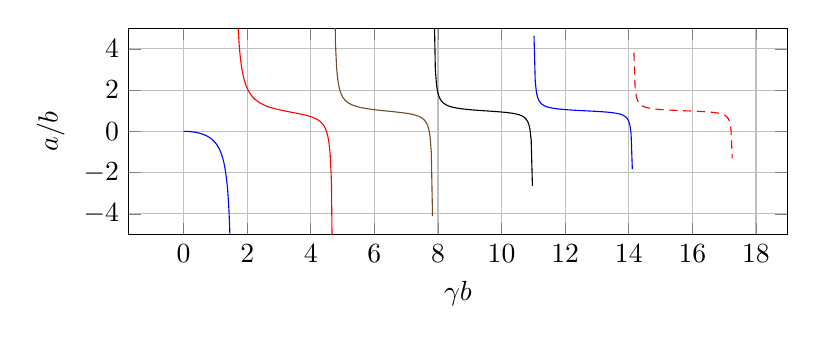
\begin{tikzpicture}
\begin{axis}[width=.82\textwidth,height=4.2cm,xlabel={$\gamma b$},ylabel={$a/b$},grid=major,legend style={font=\small},ymin=-5,ymax=5]
\addplot+[mark=none] coordinates{(0.0001,-3.33333339e-09) (0.0194212041,-0.000125746695) (0.0387424082,-0.000500625303) (0.0580636123,-0.00112531192) (0.0773848163,-0.00200092969) (0.0967060204,-0.00312905723) (0.116027225,-0.00451173587) (0.135348429,-0.00615147904) (0.154669633,-0.00805128391) (0.173990837,-0.0102146454) (0.193312041,-0.0126455725) (0.212633245,-0.0153486075) (0.231954449,-0.0183288479) (0.251275653,-0.0215919711) (0.270596857,-0.0251442626) (0.289918061,-0.0289926473) (0.309239265,-0.0331447253) (0.328560469,-0.0376088112) (0.347881674,-0.0423939778) (0.367202878,-0.0475101059) (0.386524082,-0.0529679379) (0.405845286,-0.0587791393) (0.42516649,-0.0649563655) (0.444487694,-0.0715133371) (0.463808898,-0.0784649231) (0.483130102,-0.0858272338) (0.502451306,-0.0936177243) (0.52177251,-0.10185531) (0.541093714,-0.110560493) (0.560414918,-0.119755512) (0.579736123,-0.129464497) (0.599057327,-0.139713654) (0.618378531,-0.150531466) (0.637699735,-0.161948926) (0.657020939,-0.17399979) (0.676342143,-0.186720875) (0.695663347,-0.200152384) (0.714984551,-0.214338288) (0.734305755,-0.229326752) (0.753626959,-0.245170628) (0.772948163,-0.26192801) (0.792269367,-0.279662889) (0.811590572,-0.29844589) (0.830911776,-0.318355135) (0.85023298,-0.339477246) (0.869554184,-0.361908508) (0.888875388,-0.385756231) (0.908196592,-0.41114036) (0.927517796,-0.438195359) (0.946839,-0.467072458) (0.966160204,-0.497942332) (0.985481408,-0.530998295) (1.00480261,-0.566460169) (1.02412382,-0.604578961) (1.04344502,-0.64564257) (1.06276622,-0.689982797) (1.08208743,-0.737984024) (1.10140863,-0.790094025) (1.12072984,-0.846837575) (1.14005104,-0.908833707) (1.15937225,-0.976817849) (1.17869345,-1.05167049) (1.19801465,-1.13445477) (1.21733586,-1.22646641) (1.23665706,-1.3293009) (1.25597827,-1.44494557) (1.27529947,-1.5759076) (1.29462067,-1.72539592) (1.31394188,-1.8975851) (1.33326308,-2.0980081) (1.35258429,-2.33415764) (1.37190549,-2.61643809) (1.39122669,-2.9597319) (1.4105479,-3.38609919) (1.4298691,-3.92969808) (1.44919031,-4.64639556) (1.46851151,-5.63427105) (1.48783271,-7.08277015) (1.50715392,-9.41139406) (1.52647512,-13.7711469) (1.54579633,-24.8712391)};
\addplot+[mark=none] coordinates{(1.59579633,26.0606331) (1.63444123,10.6001955) (1.67308614,6.82278676) (1.71173105,5.11772798) (1.75037596,4.14707891) (1.78902087,3.5206316) (1.82766578,3.08299901) (1.86631068,2.76007526) (1.90495559,2.51203549) (1.9436005,2.31556793) (1.98224541,2.15611893) (2.02089032,2.0241331) (2.05953522,1.91307716) (2.09818013,1.81833261) (2.13682504,1.73654208) (2.17546995,1.66520626) (2.21411486,1.60242612) (2.25275977,1.54673279) (2.29140467,1.49697218) (2.33004958,1.4522248) (2.36869449,1.41174891) (2.4073394,1.37493942) (2.44598431,1.34129765) (2.48462921,1.31040879) (2.52327412,1.28192482) (2.56191903,1.25555143) (2.60056394,1.2310379) (2.63920885,1.20816912) (2.67785376,1.18675931) (2.71649866,1.16664702) (2.75514357,1.14769105) (2.79378848,1.12976719) (2.83243339,1.11276549) (2.8710783,1.09658809) (2.9097232,1.08114729) (2.94836811,1.06636408) (2.98701302,1.05216674) (3.02565793,1.03848979) (3.06430284,1.02527299) (3.10294775,1.01246046) (3.14159265,1) (3.18023756,0.987842368) (3.21888247,0.975940691) (3.25752738,0.964249893) (3.29617229,0.952726156) (3.33481719,0.9413264) (3.3734621,0.930007761) (3.41210701,0.91872706) (3.45075192,0.907440245) (3.48939683,0.896101793) (3.52804174,0.88466405) (3.56668664,0.873076487) (3.60533155,0.861284847) (3.64397646,0.849230152) (3.68262137,0.836847513) (3.72126628,0.824064706) (3.75991118,0.810800427) (3.79855609,0.79696213) (3.837201,0.782443325) (3.87584591,0.767120145) (3.91449082,0.750846938) (3.95313573,0.733450539) (3.99178063,0.714722708) (4.03042554,0.694410027) (4.06907045,0.672200166) (4.10771536,0.647702895) (4.14636027,0.620423343) (4.18500517,0.589723512) (4.22365008,0.554765539) (4.26229499,0.514425756) (4.3009399,0.46716032) (4.33958481,0.4107873) (4.37822972,0.342117556) (4.41687462,0.256296015) (4.45551953,0.145548355) (4.49416444,-0.0034039901) (4.53280935,-0.215266479) (4.57145426,-0.54183821) (4.61009916,-1.11319182) (4.64874407,-2.37531064) (4.68738898,-7.53175755)};
\addplot+[mark=none] coordinates{(4.73738898,9.4417105) (4.77603389,4.28535259) (4.8146788,3.02340057) (4.8533237,2.45229193) (4.89196861,2.12604387) (4.93061352,1.91458447) (4.96925843,1.76611552) (5.00790334,1.65593264) (5.04654825,1.57075853) (5.08519315,1.50282033) (5.12383806,1.44726461) (5.16248297,1.40090412) (5.20112788,1.36155899) (5.23977279,1.32768772) (5.27841769,1.2981692) (5.3170626,1.27216836) (5.35570751,1.24905031) (5.39435242,1.22832354) (5.43299733,1.2096015) (5.47164224,1.19257586) (5.51028714,1.17699756) (5.54893205,1.16266309) (5.58757696,1.14940442) (5.62622187,1.13708147) (5.66486678,1.1255764) (5.70351168,1.11478929) (5.74215659,1.1046347) (5.7808015,1.09503903) (5.81944641,1.08593843) (5.85809132,1.07727712) (5.89673623,1.06900598) (5.93538113,1.06108152) (5.97402604,1.05346491) (6.01267095,1.04612126) (6.05131586,1.03901898) (6.08996077,1.03212923) (6.12860567,1.02542548) (6.16725058,1.01888312) (6.20589549,1.01247912) (6.2445404,1.00619167) (6.28318531,1) (6.32183022,0.993884025) (6.36047512,0.987824166) (6.39912003,0.981801099) (6.43776494,0.975795523) (6.47640985,0.969787933) (6.51505476,0.963758376) (6.55369966,0.957686195) (6.59234457,0.951549749) (6.63098948,0.945326097) (6.66963439,0.938990652) (6.7082793,0.932516763) (6.74692421,0.925875243) (6.78556911,0.919033796) (6.82421402,0.911956332) (6.86285893,0.904602137) (6.90150384,0.896924843) (6.94014875,0.888871152) (6.97879365,0.880379227) (7.01743856,0.871376653) (7.05608347,0.861777801) (7.09472838,0.851480403) (7.13337329,0.840361029) (7.1720182,0.828269032) (7.2106631,0.815018314) (7.24930801,0.800375949) (7.28795292,0.78404614) (7.32659783,0.765647131) (7.36524274,0.744677177) (7.40388764,0.720462983) (7.44253255,0.692079084) (7.48117746,0.658217106) (7.51982237,0.616964294) (7.55846728,0.565408285) (7.59711218,0.498885115) (7.63575709,0.409428237) (7.674402,0.28221492) (7.71304691,0.0861662157) (7.75169182,-0.256760984) (7.79033673,-1.01415624) (7.82898163,-4.10815687)};
\addplot+[mark=none] coordinates{(7.87898163,6.07574052) (7.91762654,2.98177512) (7.95627145,2.22444589) (7.99491636,1.88161558) (8.03356127,1.68569481) (8.07220617,1.55864065) (8.11085108,1.46937442) (8.14949599,1.40307367) (8.1881409,1.35177222) (8.22678581,1.3108065) (8.26543072,1.27726461) (8.30407562,1.24923432) (8.34272053,1.22540783) (8.38136544,1.20486032) (8.42001035,1.1869192) (8.45865526,1.17108349) (8.49730016,1.15697228) (8.53594507,1.14429072) (8.57458998,1.13280686) (8.61323489,1.12233571) (8.6518798,1.1127278) (8.69052471,1.10386098) (8.72916961,1.09563438) (8.76781452,1.08796385) (8.80645943,1.08077861) (8.84510434,1.07401858) (8.88374925,1.06763235) (8.92239415,1.0615756) (8.96103906,1.05580984) (8.99968397,1.05030137) (9.03832888,1.0450205) (9.07697379,1.03994085) (9.1156187,1.03503885) (9.1542636,1.0302932) (9.19290851,1.0256846) (9.23155342,1.02119532) (9.27019833,1.016809) (9.30884324,1.01251036) (9.34748814,1.00828502) (9.38613305,1.00411929) (9.42477796,1) (9.46342287,0.995914358) (9.50206778,0.991849765) (9.54071269,0.987793684) (9.57935759,0.983733488) (9.6180025,0.979656303) (9.65664741,0.975548847) (9.69529232,0.971397255) (9.73393723,0.96718689) (9.77258213,0.962902121) (9.81122704,0.95852608) (9.84987195,0.954040377) (9.88851686,0.94942476) (9.92716177,0.944656712) (9.96580668,0.939710968) (10.0044516,0.934558924) (10.0430965,0.929167902) (10.0817414,0.923500246) (10.1203863,0.917512171) (10.1590312,0.911152312) (10.1976761,0.90435984) (10.236321,0.897062021) (10.2749659,0.889170984) (10.3136108,0.880579397) (10.3522558,0.871154592) (10.3909007,0.860730434) (10.4295456,0.849095864) (10.4681905,0.835978412) (10.5068354,0.821019889) (10.5454803,0.803739554) (10.5841252,0.783476537) (10.6227701,0.75929645) (10.661415,0.729833192) (10.7000599,0.693006649) (10.7387048,0.645485554) (10.7773497,0.581579643) (10.8159947,0.49070137) (10.8546396,0.350651599) (10.8932845,0.105685355) (10.9319294,-0.435332664) (10.9705743,-2.6453576)};
\addplot+[mark=none] coordinates{(11.0205743,4.62881872) (11.0592192,2.41881222) (11.0978641,1.87782872) (11.136509,1.63291314) (11.1751539,1.49293024) (11.2137988,1.40213514) (11.2524437,1.33832882) (11.2910886,1.29092387) (11.3297336,1.2542302) (11.3683785,1.22491673) (11.4070234,1.20090355) (11.4456683,1.1808248) (11.4843132,1.16374637) (11.5229581,1.14900768) (11.561603,1.13612832) (11.6002479,1.12475046) (11.6388928,1.11460202) (11.6775377,1.10547237) (11.7161826,1.09719585) (11.7548275,1.08964029) (11.7934725,1.08269891) (11.8321174,1.07628444) (11.8707623,1.07032478) (11.9094072,1.06475979) (11.9480521,1.05953888) (11.986697,1.05461906) (12.0253419,1.04996356) (12.0639868,1.04554065) (12.1026317,1.04132276) (12.1412766,1.03728573) (12.1799215,1.03340826) (12.2185664,1.02967141) (12.2572113,1.02605819) (12.2958563,1.02255329) (12.3345012,1.01914274) (12.3731461,1.01581374) (12.411791,1.01255441) (12.4504359,1.00935364) (12.4890808,1.00620094) (12.5277257,1.00308629) (12.5663706,1) (12.6050155,0.996932637) (12.6436604,0.993874868) (12.6823053,0.990817367) (12.7209502,0.9877507) (12.7595952,0.984665209) (12.7982401,0.981550888) (12.836885,0.978397254) (12.8755299,0.975193196) (12.9141748,0.971926811) (12.9528197,0.968585215) (12.9914646,0.965154321) (13.0301095,0.961618579) (13.0687544,0.957960663) (13.1073993,0.954161095) (13.1460442,0.950197789) (13.1846891,0.946045479) (13.2233341,0.941675017) (13.261979,0.93705248) (13.3006239,0.932138038) (13.3392688,0.926884495) (13.3779137,0.921235387) (13.4165586,0.915122469) (13.4552035,0.908462356) (13.4938484,0.901151949) (13.5324933,0.893062114) (13.5711382,0.884028772) (13.6097831,0.873840075) (13.648428,0.862217498) (13.687073,0.848787197) (13.7257179,0.833035222) (13.7643628,0.814234881) (13.8030077,0.791323708) (13.8416526,0.762683882) (13.8802975,0.725724467) (13.9189424,0.676019743) (13.9575873,0.605334995) (13.9962322,0.496404265) (14.0348771,0.305870386) (14.073522,-0.114927399) (14.1121669,-1.83384306)};
\addplot+[mark=none] coordinates{(14.1621669,3.82383808) (14.2008118,2.10493368) (14.2394568,1.68415699) (14.2781017,1.49365406) (14.3167466,1.38476418) (14.3553915,1.31413024) (14.3940364,1.26448634) (14.4326813,1.22759785) (14.4713262,1.19903915) (14.5099711,1.17621941) (14.548616,1.15752092) (14.5872609,1.14188138) (14.6259058,1.12857423) (14.6645507,1.1170857) (14.7031957,1.10704214) (14.7418406,1.09816523) (14.7804855,1.09024336) (14.8191304,1.08311268) (14.8577753,1.07664434) (14.8964202,1.07073553) (14.9350651,1.06530319) (14.97371,1.06027941) (15.0123549,1.05560811) (15.0509998,1.05124249) (15.0896447,1.04714316) (15.1282896,1.04327668) (15.1669346,1.03961439) (15.2055795,1.03613159) (15.2442244,1.03280679) (15.2828693,1.02962117) (15.3215142,1.02655808) (15.3601591,1.02360276) (15.398804,1.02074192) (15.4374489,1.01796359) (15.4760938,1.01525683) (15.5147387,1.0126116) (15.5533836,1.01001857) (15.5920285,1.00746901) (15.6306735,1.00495462) (15.6693184,1.00246751) (15.7079633,1) (15.7466082,0.997544604) (15.7852531,0.995093896) (15.823898,0.992640438) (15.8625429,0.990176686) (15.9011878,0.987694898) (15.9398327,0.985187036) (15.9784776,0.982644656) (16.0171225,0.980058793) (16.0557674,0.977419823) (16.0944123,0.97471731) (16.1330573,0.971939826) (16.1717022,0.969074739) (16.2103471,0.966107957) (16.248992,0.963023624) (16.2876369,0.959803741) (16.3262818,0.956427704) (16.3649267,0.952871727) (16.4035716,0.949108114) (16.4422165,0.945104334) (16.4808614,0.940821821) (16.5195063,0.936214426) (16.5581512,0.931226358) (16.5967962,0.925789434) (16.6354411,0.919819342) (16.674086,0.913210461) (16.7127309,0.905828582) (16.7513758,0.897500406) (16.7900207,0.887998079) (16.8286656,0.877015759) (16.8673105,0.864132967) (16.9059554,0.848755162) (16.9446003,0.830013077) (16.9832452,0.806583064) (17.0218901,0.776345285) (17.0605351,0.735678716) (17.09918,0.677845881) (17.1378249,0.588720103) (17.1764698,0.432827353) (17.2151147,0.0885361146) (17.2537596,-1.3178523)};
\end{axis}\end{tikzpicture}\end{center}
\begin{center}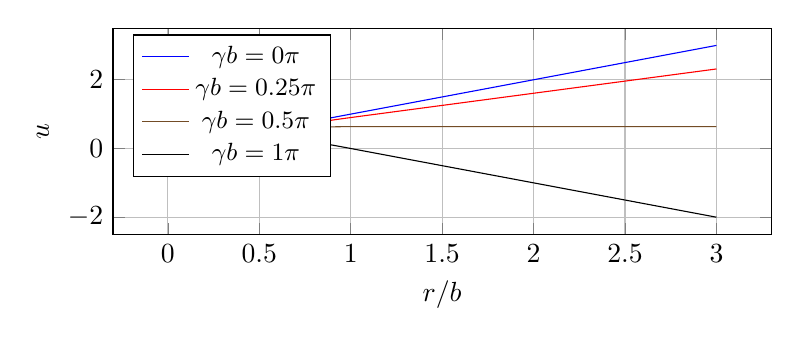
\begin{tikzpicture}
\begin{axis}[width=.82\textwidth,height=4.2cm,xlabel={$r/b$},ylabel={$u$},grid=major,legend style={font=\small},legend pos=north west]
\addplot+[mark=none] coordinates{(0,0) (0.0166666667,0.0166666667) (0.0333333333,0.0333333333) (0.05,0.05) (0.0666666667,0.0666666667) (0.0833333333,0.0833333333) (0.1,0.1) (0.116666667,0.116666667) (0.133333333,0.133333333) (0.15,0.15) (0.166666667,0.166666667) (0.183333333,0.183333333) (0.2,0.2) (0.216666667,0.216666667) (0.233333333,0.233333333) (0.25,0.25) (0.266666667,0.266666667) (0.283333333,0.283333333) (0.3,0.3) (0.316666667,0.316666667) (0.333333333,0.333333333) (0.35,0.35) (0.366666667,0.366666667) (0.383333333,0.383333333) (0.4,0.4) (0.416666667,0.416666667) (0.433333333,0.433333333) (0.45,0.45) (0.466666667,0.466666667) (0.483333333,0.483333333) (0.5,0.5) (0.516666667,0.516666667) (0.533333333,0.533333333) (0.55,0.55) (0.566666667,0.566666667) (0.583333333,0.583333333) (0.6,0.6) (0.616666667,0.616666667) (0.633333333,0.633333333) (0.65,0.65) (0.666666667,0.666666667) (0.683333333,0.683333333) (0.7,0.7) (0.716666667,0.716666667) (0.733333333,0.733333333) (0.75,0.75) (0.766666667,0.766666667) (0.783333333,0.783333333) (0.8,0.8) (0.816666667,0.816666667) (0.833333333,0.833333333) (0.85,0.85) (0.866666667,0.866666667) (0.883333333,0.883333333) (0.9,0.9) (0.916666667,0.916666667) (0.933333333,0.933333333) (0.95,0.95) (0.966666667,0.966666667) (0.983333333,0.983333333) (1,1) (1.01666667,1.01666667) (1.03333333,1.03333333) (1.05,1.05) (1.06666667,1.06666667) (1.08333333,1.08333333) (1.1,1.1) (1.11666667,1.11666667) (1.13333333,1.13333333) (1.15,1.15) (1.16666667,1.16666667) (1.18333333,1.18333333) (1.2,1.2) (1.21666667,1.21666667) (1.23333333,1.23333333) (1.25,1.25) (1.26666667,1.26666667) (1.28333333,1.28333333) (1.3,1.3) (1.31666667,1.31666667) (1.33333333,1.33333333) (1.35,1.35) (1.36666667,1.36666667) (1.38333333,1.38333333) (1.4,1.4) (1.41666667,1.41666667) (1.43333333,1.43333333) (1.45,1.45) (1.46666667,1.46666667) (1.48333333,1.48333333) (1.5,1.5) (1.51666667,1.51666667) (1.53333333,1.53333333) (1.55,1.55) (1.56666667,1.56666667) (1.58333333,1.58333333) (1.6,1.6) (1.61666667,1.61666667) (1.63333333,1.63333333) (1.65,1.65) (1.66666667,1.66666667) (1.68333333,1.68333333) (1.7,1.7) (1.71666667,1.71666667) (1.73333333,1.73333333) (1.75,1.75) (1.76666667,1.76666667) (1.78333333,1.78333333) (1.8,1.8) (1.81666667,1.81666667) (1.83333333,1.83333333) (1.85,1.85) (1.86666667,1.86666667) (1.88333333,1.88333333) (1.9,1.9) (1.91666667,1.91666667) (1.93333333,1.93333333) (1.95,1.95) (1.96666667,1.96666667) (1.98333333,1.98333333) (2,2) (2.01666667,2.01666667) (2.03333333,2.03333333) (2.05,2.05) (2.06666667,2.06666667) (2.08333333,2.08333333) (2.1,2.1) (2.11666667,2.11666667) (2.13333333,2.13333333) (2.15,2.15) (2.16666667,2.16666667) (2.18333333,2.18333333) (2.2,2.2) (2.21666667,2.21666667) (2.23333333,2.23333333) (2.25,2.25) (2.26666667,2.26666667) (2.28333333,2.28333333) (2.3,2.3) (2.31666667,2.31666667) (2.33333333,2.33333333) (2.35,2.35) (2.36666667,2.36666667) (2.38333333,2.38333333) (2.4,2.4) (2.41666667,2.41666667) (2.43333333,2.43333333) (2.45,2.45) (2.46666667,2.46666667) (2.48333333,2.48333333) (2.5,2.5) (2.51666667,2.51666667) (2.53333333,2.53333333) (2.55,2.55) (2.56666667,2.56666667) (2.58333333,2.58333333) (2.6,2.6) (2.61666667,2.61666667) (2.63333333,2.63333333) (2.65,2.65) (2.66666667,2.66666667) (2.68333333,2.68333333) (2.7,2.7) (2.71666667,2.71666667) (2.73333333,2.73333333) (2.75,2.75) (2.76666667,2.76666667) (2.78333333,2.78333333) (2.8,2.8) (2.81666667,2.81666667) (2.83333333,2.83333333) (2.85,2.85) (2.86666667,2.86666667) (2.88333333,2.88333333) (2.9,2.9) (2.91666667,2.91666667) (2.93333333,2.93333333) (2.95,2.95) (2.96666667,2.96666667) (2.98333333,2.98333333) (3,3)};
\addlegendentry{$\gamma b=0\pi$}
\addplot+[mark=none] coordinates{(0,0) (0.0166666667,0.0166661907) (0.0333333333,0.0333295257) (0.05,0.0499871499) (0.0666666667,0.0666362091) (0.0833333333,0.0832738505) (0.1,0.0998972233) (0.116666667,0.116503479) (0.133333333,0.133089773) (0.15,0.149653262) (0.166666667,0.16619111) (0.183333333,0.182700481) (0.2,0.199178547) (0.216666667,0.215622485) (0.233333333,0.232029478) (0.25,0.248396713) (0.266666667,0.264721387) (0.283333333,0.281000702) (0.3,0.297231869) (0.316666667,0.313412107) (0.333333333,0.329538643) (0.35,0.345608715) (0.366666667,0.361619568) (0.383333333,0.37756846) (0.4,0.393452657) (0.416666667,0.409269438) (0.433333333,0.425016093) (0.45,0.440689924) (0.466666667,0.456288245) (0.483333333,0.471808383) (0.5,0.487247679) (0.516666667,0.502603488) (0.533333333,0.517873178) (0.55,0.533054134) (0.566666667,0.548143753) (0.583333333,0.563139451) (0.6,0.578038657) (0.616666667,0.59283882) (0.633333333,0.607537403) (0.65,0.622131887) (0.666666667,0.636619772) (0.683333333,0.650998576) (0.7,0.665265835) (0.716666667,0.679419103) (0.733333333,0.693455957) (0.75,0.707373991) (0.766666667,0.721170819) (0.783333333,0.734844079) (0.8,0.748391427) (0.816666667,0.761810542) (0.833333333,0.775099125) (0.85,0.788254898) (0.866666667,0.801275608) (0.883333333,0.814159024) (0.9,0.826902937) (0.916666667,0.839505165) (0.933333333,0.851963549) (0.95,0.864275952) (0.966666667,0.876440267) (0.983333333,0.888454407) (1,0.900316316) (1.01666667,0.912101429) (1.03333333,0.923886542) (1.05,0.935671655) (1.06666667,0.947456768) (1.08333333,0.959241881) (1.1,0.971026994) (1.11666667,0.982812107) (1.13333333,0.99459722) (1.15,1.00638233) (1.16666667,1.01816745) (1.18333333,1.02995256) (1.2,1.04173767) (1.21666667,1.05352279) (1.23333333,1.0653079) (1.25,1.07709301) (1.26666667,1.08887812) (1.28333333,1.10066324) (1.3,1.11244835) (1.31666667,1.12423346) (1.33333333,1.13601858) (1.35,1.14780369) (1.36666667,1.1595888) (1.38333333,1.17137392) (1.4,1.18315903) (1.41666667,1.19494414) (1.43333333,1.20672925) (1.45,1.21851437) (1.46666667,1.23029948) (1.48333333,1.24208459) (1.5,1.25386971) (1.51666667,1.26565482) (1.53333333,1.27743993) (1.55,1.28922505) (1.56666667,1.30101016) (1.58333333,1.31279527) (1.6,1.32458038) (1.61666667,1.3363655) (1.63333333,1.34815061) (1.65,1.35993572) (1.66666667,1.37172084) (1.68333333,1.38350595) (1.7,1.39529106) (1.71666667,1.40707618) (1.73333333,1.41886129) (1.75,1.4306464) (1.76666667,1.44243152) (1.78333333,1.45421663) (1.8,1.46600174) (1.81666667,1.47778685) (1.83333333,1.48957197) (1.85,1.50135708) (1.86666667,1.51314219) (1.88333333,1.52492731) (1.9,1.53671242) (1.91666667,1.54849753) (1.93333333,1.56028265) (1.95,1.57206776) (1.96666667,1.58385287) (1.98333333,1.59563798) (2,1.6074231) (2.01666667,1.61920821) (2.03333333,1.63099332) (2.05,1.64277844) (2.06666667,1.65456355) (2.08333333,1.66634866) (2.1,1.67813378) (2.11666667,1.68991889) (2.13333333,1.701704) (2.15,1.71348911) (2.16666667,1.72527423) (2.18333333,1.73705934) (2.2,1.74884445) (2.21666667,1.76062957) (2.23333333,1.77241468) (2.25,1.78419979) (2.26666667,1.79598491) (2.28333333,1.80777002) (2.3,1.81955513) (2.31666667,1.83134024) (2.33333333,1.84312536) (2.35,1.85491047) (2.36666667,1.86669558) (2.38333333,1.8784807) (2.4,1.89026581) (2.41666667,1.90205092) (2.43333333,1.91383604) (2.45,1.92562115) (2.46666667,1.93740626) (2.48333333,1.94919137) (2.5,1.96097649) (2.51666667,1.9727616) (2.53333333,1.98454671) (2.55,1.99633183) (2.56666667,2.00811694) (2.58333333,2.01990205) (2.6,2.03168717) (2.61666667,2.04347228) (2.63333333,2.05525739) (2.65,2.06704251) (2.66666667,2.07882762) (2.68333333,2.09061273) (2.7,2.10239784) (2.71666667,2.11418296) (2.73333333,2.12596807) (2.75,2.13775318) (2.76666667,2.1495383) (2.78333333,2.16132341) (2.8,2.17310852) (2.81666667,2.18489364) (2.83333333,2.19667875) (2.85,2.20846386) (2.86666667,2.22024897) (2.88333333,2.23203409) (2.9,2.2438192) (2.91666667,2.25560431) (2.93333333,2.26738943) (2.95,2.27917454) (2.96666667,2.29095965) (2.98333333,2.30274477) (3,2.31452988)};
\addlegendentry{$\gamma b=0.25\pi$}
\addplot+[mark=none] coordinates{(0,0) (0.0166666667,0.0166647629) (0.0333333333,0.0333181046) (0.05,0.0499486117) (0.0666666667,0.0665448865) (0.0833333333,0.0830955548) (0.1,0.0995892735) (0.116666667,0.116014739) (0.133333333,0.132360693) (0.15,0.148615934) (0.166666667,0.164769322) (0.183333333,0.180809784) (0.2,0.196726329) (0.216666667,0.212508047) (0.233333333,0.228144122) (0.25,0.24362384) (0.266666667,0.258936589) (0.283333333,0.274071876) (0.3,0.289019329) (0.316666667,0.303768701) (0.333333333,0.318309886) (0.35,0.332632917) (0.366666667,0.346727978) (0.383333333,0.36058541) (0.4,0.374195714) (0.416666667,0.387549562) (0.433333333,0.400637804) (0.45,0.413451469) (0.466666667,0.425981774) (0.483333333,0.438220133) (0.5,0.450158158) (0.516666667,0.461787667) (0.533333333,0.47310069) (0.55,0.484089473) (0.566666667,0.494746485) (0.583333333,0.505064423) (0.6,0.515036215) (0.616666667,0.524655027) (0.633333333,0.533914266) (0.65,0.542807587) (0.666666667,0.551328895) (0.683333333,0.55947235) (0.7,0.567232371) (0.716666667,0.574603638) (0.733333333,0.581581101) (0.75,0.588159978) (0.766666667,0.594335759) (0.783333333,0.600104211) (0.8,0.605461383) (0.816666667,0.610403601) (0.833333333,0.61492748) (0.85,0.619029917) (0.866666667,0.622708103) (0.883333333,0.625959515) (0.9,0.628781927) (0.916666667,0.631173402) (0.933333333,0.633132303) (0.95,0.634657286) (0.966666667,0.635747307) (0.983333333,0.636401619) (1,0.636619772) (1.01666667,0.636619772) (1.03333333,0.636619772) (1.05,0.636619772) (1.06666667,0.636619772) (1.08333333,0.636619772) (1.1,0.636619772) (1.11666667,0.636619772) (1.13333333,0.636619772) (1.15,0.636619772) (1.16666667,0.636619772) (1.18333333,0.636619772) (1.2,0.636619772) (1.21666667,0.636619772) (1.23333333,0.636619772) (1.25,0.636619772) (1.26666667,0.636619772) (1.28333333,0.636619772) (1.3,0.636619772) (1.31666667,0.636619772) (1.33333333,0.636619772) (1.35,0.636619772) (1.36666667,0.636619772) (1.38333333,0.636619772) (1.4,0.636619772) (1.41666667,0.636619772) (1.43333333,0.636619772) (1.45,0.636619772) (1.46666667,0.636619772) (1.48333333,0.636619772) (1.5,0.636619772) (1.51666667,0.636619772) (1.53333333,0.636619772) (1.55,0.636619772) (1.56666667,0.636619772) (1.58333333,0.636619772) (1.6,0.636619772) (1.61666667,0.636619772) (1.63333333,0.636619772) (1.65,0.636619772) (1.66666667,0.636619772) (1.68333333,0.636619772) (1.7,0.636619772) (1.71666667,0.636619772) (1.73333333,0.636619772) (1.75,0.636619772) (1.76666667,0.636619772) (1.78333333,0.636619772) (1.8,0.636619772) (1.81666667,0.636619772) (1.83333333,0.636619772) (1.85,0.636619772) (1.86666667,0.636619772) (1.88333333,0.636619772) (1.9,0.636619772) (1.91666667,0.636619772) (1.93333333,0.636619772) (1.95,0.636619772) (1.96666667,0.636619772) (1.98333333,0.636619772) (2,0.636619772) (2.01666667,0.636619772) (2.03333333,0.636619772) (2.05,0.636619772) (2.06666667,0.636619772) (2.08333333,0.636619772) (2.1,0.636619772) (2.11666667,0.636619772) (2.13333333,0.636619772) (2.15,0.636619772) (2.16666667,0.636619772) (2.18333333,0.636619772) (2.2,0.636619772) (2.21666667,0.636619772) (2.23333333,0.636619772) (2.25,0.636619772) (2.26666667,0.636619772) (2.28333333,0.636619772) (2.3,0.636619772) (2.31666667,0.636619772) (2.33333333,0.636619772) (2.35,0.636619772) (2.36666667,0.636619772) (2.38333333,0.636619772) (2.4,0.636619772) (2.41666667,0.636619772) (2.43333333,0.636619772) (2.45,0.636619772) (2.46666667,0.636619772) (2.48333333,0.636619772) (2.5,0.636619772) (2.51666667,0.636619772) (2.53333333,0.636619772) (2.55,0.636619772) (2.56666667,0.636619772) (2.58333333,0.636619772) (2.6,0.636619772) (2.61666667,0.636619772) (2.63333333,0.636619772) (2.65,0.636619772) (2.66666667,0.636619772) (2.68333333,0.636619772) (2.7,0.636619772) (2.71666667,0.636619772) (2.73333333,0.636619772) (2.75,0.636619772) (2.76666667,0.636619772) (2.78333333,0.636619772) (2.8,0.636619772) (2.81666667,0.636619772) (2.83333333,0.636619772) (2.85,0.636619772) (2.86666667,0.636619772) (2.88333333,0.636619772) (2.9,0.636619772) (2.91666667,0.636619772) (2.93333333,0.636619772) (2.95,0.636619772) (2.96666667,0.636619772) (2.98333333,0.636619772) (3,0.636619772)};
\addlegendentry{$\gamma b=0.5\pi$}
\addplot+[mark=none] coordinates{(0,0) (0.0166666667,0.0166590523) (0.0333333333,0.0332724432) (0.05,0.0497946368) (0.0666666667,0.0661803466) (0.0833333333,0.0823846608) (0.1,0.0983631643) (0.116666667,0.114072061) (0.133333333,0.129468295) (0.15,0.144509664) (0.166666667,0.159154943) (0.183333333,0.173363989) (0.2,0.187097857) (0.216666667,0.200318902) (0.233333333,0.212990887) (0.25,0.225079079) (0.266666667,0.236550345) (0.283333333,0.247373243) (0.3,0.257518107) (0.316666667,0.266957133) (0.333333333,0.275664448) (0.35,0.283616185) (0.366666667,0.290790551) (0.383333333,0.297167879) (0.4,0.302730691) (0.416666667,0.30746374) (0.433333333,0.311354051) (0.45,0.314390963) (0.466666667,0.316566151) (0.483333333,0.317873654) (0.5,0.318309886) (0.516666667,0.317873654) (0.533333333,0.316566151) (0.55,0.314390963) (0.566666667,0.311354051) (0.583333333,0.30746374) (0.6,0.302730691) (0.616666667,0.297167879) (0.633333333,0.290790551) (0.65,0.283616185) (0.666666667,0.275664448) (0.683333333,0.266957133) (0.7,0.257518107) (0.716666667,0.247373243) (0.733333333,0.236550345) (0.75,0.225079079) (0.766666667,0.212990887) (0.783333333,0.200318902) (0.8,0.187097857) (0.816666667,0.173363989) (0.833333333,0.159154943) (0.85,0.144509664) (0.866666667,0.129468295) (0.883333333,0.114072061) (0.9,0.0983631643) (0.916666667,0.0823846608) (0.933333333,0.0661803466) (0.95,0.0497946368) (0.966666667,0.0332724432) (0.983333333,0.0166590523) (1,3.89817183e-17) (1.01666667,-0.0166666667) (1.03333333,-0.0333333333) (1.05,-0.05) (1.06666667,-0.0666666667) (1.08333333,-0.0833333333) (1.1,-0.1) (1.11666667,-0.116666667) (1.13333333,-0.133333333) (1.15,-0.15) (1.16666667,-0.166666667) (1.18333333,-0.183333333) (1.2,-0.2) (1.21666667,-0.216666667) (1.23333333,-0.233333333) (1.25,-0.25) (1.26666667,-0.266666667) (1.28333333,-0.283333333) (1.3,-0.3) (1.31666667,-0.316666667) (1.33333333,-0.333333333) (1.35,-0.35) (1.36666667,-0.366666667) (1.38333333,-0.383333333) (1.4,-0.4) (1.41666667,-0.416666667) (1.43333333,-0.433333333) (1.45,-0.45) (1.46666667,-0.466666667) (1.48333333,-0.483333333) (1.5,-0.5) (1.51666667,-0.516666667) (1.53333333,-0.533333333) (1.55,-0.55) (1.56666667,-0.566666667) (1.58333333,-0.583333333) (1.6,-0.6) (1.61666667,-0.616666667) (1.63333333,-0.633333333) (1.65,-0.65) (1.66666667,-0.666666667) (1.68333333,-0.683333333) (1.7,-0.7) (1.71666667,-0.716666667) (1.73333333,-0.733333333) (1.75,-0.75) (1.76666667,-0.766666667) (1.78333333,-0.783333333) (1.8,-0.8) (1.81666667,-0.816666667) (1.83333333,-0.833333333) (1.85,-0.85) (1.86666667,-0.866666667) (1.88333333,-0.883333333) (1.9,-0.9) (1.91666667,-0.916666667) (1.93333333,-0.933333333) (1.95,-0.95) (1.96666667,-0.966666667) (1.98333333,-0.983333333) (2,-1) (2.01666667,-1.01666667) (2.03333333,-1.03333333) (2.05,-1.05) (2.06666667,-1.06666667) (2.08333333,-1.08333333) (2.1,-1.1) (2.11666667,-1.11666667) (2.13333333,-1.13333333) (2.15,-1.15) (2.16666667,-1.16666667) (2.18333333,-1.18333333) (2.2,-1.2) (2.21666667,-1.21666667) (2.23333333,-1.23333333) (2.25,-1.25) (2.26666667,-1.26666667) (2.28333333,-1.28333333) (2.3,-1.3) (2.31666667,-1.31666667) (2.33333333,-1.33333333) (2.35,-1.35) (2.36666667,-1.36666667) (2.38333333,-1.38333333) (2.4,-1.4) (2.41666667,-1.41666667) (2.43333333,-1.43333333) (2.45,-1.45) (2.46666667,-1.46666667) (2.48333333,-1.48333333) (2.5,-1.5) (2.51666667,-1.51666667) (2.53333333,-1.53333333) (2.55,-1.55) (2.56666667,-1.56666667) (2.58333333,-1.58333333) (2.6,-1.6) (2.61666667,-1.61666667) (2.63333333,-1.63333333) (2.65,-1.65) (2.66666667,-1.66666667) (2.68333333,-1.68333333) (2.7,-1.7) (2.71666667,-1.71666667) (2.73333333,-1.73333333) (2.75,-1.75) (2.76666667,-1.76666667) (2.78333333,-1.78333333) (2.8,-1.8) (2.81666667,-1.81666667) (2.83333333,-1.83333333) (2.85,-1.85) (2.86666667,-1.86666667) (2.88333333,-1.88333333) (2.9,-1.9) (2.91666667,-1.91666667) (2.93333333,-1.93333333) (2.95,-1.95) (2.96666667,-1.96666667) (2.98333333,-1.98333333) (3,-2)};
\addlegendentry{$\gamma b=1\pi$}
\end{axis}\end{tikzpicture}\end{center}

\end{solution}
\originalsection{第4题：排斥δ壳的窄共振}
\begin{exercise}
$V=\lambda\hbar^2\delta(r-R)/(2mR)$, $\lambda\gg1$正. (a)从界面导数比求$\delta_0$. (b)求散射长度. (c)画相移与截面, 分析$kR$略低于$n\pi$的快速$\pi$变化及与硬球关系.
\end{exercise}
\begin{solution}
径向$u$连续, 跳跃$u'(R+)-u'(R-)=\lambda u(R)/R$. 内$\sin kr$, 外$\sin(kr+\delta_0)$, 令$z=kR$, 得$\cot(z+\delta_0)=\cot z+\lambda/z$. 消和角后
\[
\tan\delta_0=-\frac{\lambda\sin^2z}{z+\lambda\sin z\cos z},\qquad
 a_s=\frac{\lambda R}{1+\lambda}.
\]
$\lambda\to\infty$取固定$z$, 或有限大$\lambda$时限定$z\ll\lambda$, 除共振窗外$\delta_0\simeq-z$模$\pi$, 正是硬球,$\sigma_0=4\pi\sin^2\delta_0/k^2$. 在$z=n\pi-\epsilon$附近, 分母$\simeq n\pi-(\lambda+1)\epsilon$, 于$\epsilon\simeq n\pi/(\lambda+1)$过零, 此展开须$n\pi\ll\lambda$. $z\gg\lambda$时壳相对较弱, 不属于硬球近似. 连续选择相位时快速增加$\pi$, 截面有达到幺正峰的窄共振. 壳内几乎封闭的球井驻波$kR\simeq n\pi$变成寿命有限的准束缚态; 正排斥壳不支持真正负能束缚态. 图取有限$\lambda$展现共振, 不把arctan分支跳跃本身误作物理不连续.
\begin{center}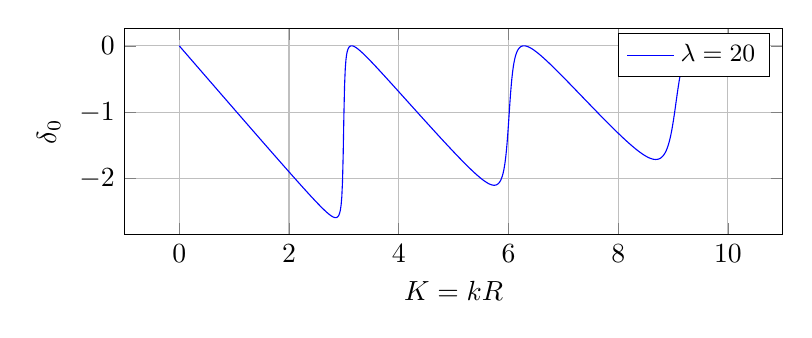
\begin{tikzpicture}
\begin{axis}[width=.82\textwidth,height=4.2cm,xlabel={$K=kR$},ylabel={$\delta_0$},grid=major,legend style={font=\small},]
\addplot+[mark=none] coordinates{(0.001,-0.000952380952) (0.01349875,-0.0128559506) (0.0259975,-0.0247595112) (0.03849625,-0.0366630542) (0.050995,-0.0485665712) (0.06349375,-0.0604700538) (0.0759925,-0.0723734935) (0.08849125,-0.0842768818) (0.10099,-0.0961802103) (0.11348875,-0.10808347) (0.1259875,-0.119986654) (0.13848625,-0.131889752) (0.150985,-0.143792756) (0.16348375,-0.155695657) (0.1759825,-0.167598447) (0.18848125,-0.179501118) (0.20098,-0.19140366) (0.21347875,-0.203306065) (0.2259775,-0.215208324) (0.23847625,-0.227110428) (0.250975,-0.239012369) (0.26347375,-0.250914137) (0.2759725,-0.262815724) (0.28847125,-0.274717121) (0.30097,-0.286618318) (0.31346875,-0.298519307) (0.3259675,-0.310420079) (0.33846625,-0.322320624) (0.350965,-0.334220933) (0.36346375,-0.346120997) (0.3759625,-0.358020806) (0.38846125,-0.369920351) (0.40096,-0.381819623) (0.41345875,-0.393718611) (0.4259575,-0.405617306) (0.43845625,-0.417515699) (0.450955,-0.429413779) (0.46345375,-0.441311536) (0.4759525,-0.453208961) (0.48845125,-0.465106044) (0.50095,-0.477002773) (0.51344875,-0.488899139) (0.5259475,-0.500795132) (0.53844625,-0.51269074) (0.550945,-0.524585953) (0.56344375,-0.53648076) (0.5759425,-0.548375151) (0.58844125,-0.560269114) (0.60094,-0.572162639) (0.61343875,-0.584055712) (0.6259375,-0.595948325) (0.63843625,-0.607840464) (0.650935,-0.619732118) (0.66343375,-0.631623275) (0.6759325,-0.643513923) (0.68843125,-0.65540405) (0.70093,-0.667293644) (0.71342875,-0.679182691) (0.7259275,-0.691071179) (0.73842625,-0.702959096) (0.750925,-0.714846427) (0.76342375,-0.726733161) (0.7759225,-0.738619282) (0.78842125,-0.750504778) (0.80092,-0.762389635) (0.81341875,-0.774273837) (0.8259175,-0.786157372) (0.83841625,-0.798040224) (0.850915,-0.809922378) (0.86341375,-0.82180382) (0.8759125,-0.833684533) (0.88841125,-0.845564503) (0.90091,-0.857443712) (0.91340875,-0.869322146) (0.9259075,-0.881199787) (0.93840625,-0.893076618) (0.950905,-0.904952623) (0.96340375,-0.916827783) (0.9759025,-0.928702082) (0.98840125,-0.940575501) (1.0009,-0.952448021) (1.01339875,-0.964319623) (1.0258975,-0.976190288) (1.03839625,-0.988059997) (1.050895,-0.999928729) (1.06339375,-1.01179646) (1.0758925,-1.02366318) (1.08839125,-1.03552886) (1.10089,-1.04739348) (1.11338875,-1.05925701) (1.1258875,-1.07111943) (1.13838625,-1.08298073) (1.150885,-1.09484087) (1.16338375,-1.10669984) (1.1758825,-1.1185576) (1.18838125,-1.13041413) (1.20088,-1.14226941) (1.21337875,-1.1541234) (1.2258775,-1.16597609) (1.23837625,-1.17782743) (1.250875,-1.18967742) (1.26337375,-1.201526) (1.2758725,-1.21337316) (1.28837125,-1.22521886) (1.30087,-1.23706307) (1.31336875,-1.24890576) (1.3258675,-1.2607469) (1.33836625,-1.27258644) (1.350865,-1.28442436) (1.36336375,-1.29626062) (1.3758625,-1.30809517) (1.38836125,-1.31992799) (1.40086,-1.33175903) (1.41335875,-1.34358825) (1.4258575,-1.35541561) (1.43835625,-1.36724106) (1.450855,-1.37906457) (1.46335375,-1.39088608) (1.4758525,-1.40270555) (1.48835125,-1.41452294) (1.50085,-1.42633818) (1.51334875,-1.43815123) (1.5258475,-1.44996203) (1.53834625,-1.46177054) (1.550845,-1.47357669) (1.56334375,-1.48538042) (1.5758425,-1.49718168) (1.58834125,-1.50898039) (1.60084,-1.52077651) (1.61333875,-1.53256995) (1.6258375,-1.54436066) (1.63833625,-1.55614856) (1.650835,-1.56793357) (1.66333375,-1.57971562) (1.6758325,-1.59149462) (1.68833125,-1.60327051) (1.70083,-1.61504318) (1.71332875,-1.62681256) (1.7258275,-1.63857855) (1.73832625,-1.65034106) (1.750825,-1.66209998) (1.76332375,-1.67385521) (1.7758225,-1.68560665) (1.78832125,-1.69735419) (1.80082,-1.7090977) (1.81331875,-1.72083708) (1.8258175,-1.73257219) (1.83831625,-1.7443029) (1.850815,-1.75602908) (1.86331375,-1.76775058) (1.8758125,-1.77946726) (1.88831125,-1.79117897) (1.90081,-1.80288553) (1.91330875,-1.81458679) (1.9258075,-1.82628256) (1.93830625,-1.83797267) (1.950805,-1.84965691) (1.96330375,-1.86133509) (1.9758025,-1.87300699) (1.98830125,-1.8846724) (2.0008,-1.89633108) (2.01329875,-1.90798277) (2.0257975,-1.91962724) (2.03829625,-1.9312642) (2.050795,-1.94289338) (2.06329375,-1.95451447) (2.0757925,-1.96612716) (2.08829125,-1.97773111) (2.10079,-1.98932598) (2.11328875,-2.0009114) (2.1257875,-2.01248696) (2.13828625,-2.02405227) (2.150785,-2.03560688) (2.16328375,-2.04715033) (2.1757825,-2.05868213) (2.18828125,-2.07020175) (2.20078,-2.08170864) (2.21327875,-2.09320222) (2.2257775,-2.10468185) (2.23827625,-2.11614686) (2.250775,-2.12759655) (2.26327375,-2.13903015) (2.2757725,-2.15044686) (2.28827125,-2.16184579) (2.30077,-2.17322602) (2.31326875,-2.18458655) (2.3257675,-2.1959263) (2.33826625,-2.20724412) (2.350765,-2.21853877) (2.36326375,-2.2298089) (2.3757625,-2.24105307) (2.38826125,-2.2522697) (2.40076,-2.2634571) (2.41325875,-2.27461343) (2.4257575,-2.28573667) (2.43825625,-2.29682465) (2.450755,-2.30787499) (2.46325375,-2.31888508) (2.4757525,-2.32985206) (2.48825125,-2.34077281) (2.50075,-2.35164387) (2.51324875,-2.36246144) (2.5257475,-2.37322131) (2.53824625,-2.38391882) (2.550745,-2.39454879) (2.56324375,-2.40510542) (2.5757425,-2.41558226) (2.58824125,-2.42597205) (2.60074,-2.43626662) (2.61323875,-2.44645673) (2.6257375,-2.45653192) (2.63823625,-2.46648025) (2.650735,-2.47628809) (2.66323375,-2.48593975) (2.6757325,-2.49541712) (2.68823125,-2.50469915) (2.70073,-2.51376127) (2.71322875,-2.5225746) (2.7257275,-2.53110494) (2.73822625,-2.53931153) (2.750725,-2.5471454) (2.76322375,-2.55454716) (2.7757225,-2.5614441) (2.78822125,-2.56774626) (2.80072,-2.57334101) (2.81321875,-2.57808543) (2.8257175,-2.5817955) (2.83821625,-2.58423019) (2.850715,-2.5850678) (2.86321375,-2.58386935) (2.8757125,-2.58002036) (2.88821125,-2.57263469) (2.90071,-2.56038844) (2.91320875,-2.54121814) (2.9257075,-2.51173845) (2.93820625,-2.46603761) (2.950705,-2.39298703) (2.96320375,-2.2698203) (2.9757025,-2.04739218) (2.98820125,-1.63865305) (3.0007,-1.06199063) (3.01319875,-0.605715918) (3.0256975,-0.351830214) (3.03819625,-0.213023536) (3.050695,-0.131835562) (3.06319375,-0.0815141297) (3.0756925,-0.0491971949) (3.08819125,-0.0281698855) (3.10069,-0.0146436509) (3.11318875,-0.00633730553) (3.1256875,-0.00180188685) (3.13818625,-7.55916523e-05) (3.150685,-0.000496131642) (3.16318375,-0.00259314952) (3.1756825,-0.00602368749) (3.18818125,-0.0105319494) (3.20068,-0.0159233548) (3.21317875,-0.0220473132) (3.2256775,-0.0287854883) (3.23817625,-0.0360436214) (3.250675,-0.0437457156) (3.26317375,-0.0518298251) (3.2756725,-0.0602449567) (3.28817125,-0.068948754) (3.30067,-0.0779057458) (3.31316875,-0.0870860025) (3.3256675,-0.0964640955) (3.33816625,-0.106018282) (3.350665,-0.115729861) (3.36316375,-0.125582659) (3.3756625,-0.135562617) (3.38816125,-0.145657456) (3.40066,-0.155856401) (3.41315875,-0.166149963) (3.4256575,-0.176529747) (3.43815625,-0.1869883) (3.450655,-0.197518984) (3.46315375,-0.208115864) (3.4756525,-0.218773619) (3.48815125,-0.229487465) (3.50065,-0.240253087) (3.51314875,-0.251066581) (3.5256475,-0.261924412) (3.53814625,-0.272823362) (3.550645,-0.283760504) (3.56314375,-0.294733163) (3.5756425,-0.305738891) (3.58814125,-0.316775446) (3.60064,-0.327840766) (3.61313875,-0.338932952) (3.6256375,-0.350050256) (3.63813625,-0.361191059) (3.650635,-0.372353866) (3.66313375,-0.383537288) (3.6756325,-0.394740038) (3.68813125,-0.405960916) (3.70063,-0.417198806) (3.71312875,-0.428452665) (3.7256275,-0.439721521) (3.73812625,-0.451004463) (3.750625,-0.462300636) (3.76312375,-0.473609239) (3.7756225,-0.484929518) (3.78812125,-0.496260766) (3.80062,-0.507602314) (3.81311875,-0.518953532) (3.8256175,-0.530313824) (3.83811625,-0.541682626) (3.850615,-0.553059405) (3.86311375,-0.564443654) (3.8756125,-0.575834892) (3.88811125,-0.587232661) (3.90061,-0.598636525) (3.91310875,-0.610046068) (3.9256075,-0.621460894) (3.93810625,-0.632880622) (3.950605,-0.64430489) (3.96310375,-0.655733349) (3.9756025,-0.667165665) (3.98810125,-0.678601515) (4.0006,-0.690040591) (4.01309875,-0.701482594) (4.0255975,-0.712927236) (4.03809625,-0.72437424) (4.050595,-0.735823335) (4.06309375,-0.74727426) (4.0755925,-0.758726763) (4.08809125,-0.770180597) (4.10059,-0.781635522) (4.11308875,-0.793091304) (4.1255875,-0.804547716) (4.13808625,-0.816004535) (4.150585,-0.827461542) (4.16308375,-0.838918523) (4.1755825,-0.850375268) (4.18808125,-0.861831571) (4.20058,-0.873287228) (4.21307875,-0.884742038) (4.2255775,-0.896195802) (4.23807625,-0.907648326) (4.250575,-0.919099415) (4.26307375,-0.930548876) (4.2755725,-0.941996518) (4.28807125,-0.95344215) (4.30057,-0.964885583) (4.31306875,-0.976326628) (4.3255675,-0.987765096) (4.33806625,-0.999200796) (4.350565,-1.01063354) (4.36306375,-1.02206314) (4.3755625,-1.0334894) (4.38806125,-1.04491214) (4.40056,-1.05633115) (4.41305875,-1.06774625) (4.4255575,-1.07915723) (4.43805625,-1.0905639) (4.450555,-1.10196606) (4.46305375,-1.1133635) (4.4755525,-1.12475602) (4.48805125,-1.13614341) (4.50055,-1.14752545) (4.51304875,-1.15890192) (4.5255475,-1.17027262) (4.53804625,-1.18163731) (4.550545,-1.19299576) (4.56304375,-1.20434774) (4.5755425,-1.21569301) (4.58804125,-1.22703132) (4.60054,-1.23836242) (4.61303875,-1.24968606) (4.6255375,-1.26100198) (4.63803625,-1.27230989) (4.650535,-1.28360952) (4.66303375,-1.29490059) (4.6755325,-1.30618281) (4.68803125,-1.31745586) (4.70053,-1.32871944) (4.71302875,-1.33997322) (4.7255275,-1.35121687) (4.73802625,-1.36245005) (4.750525,-1.3736724) (4.76302375,-1.38488356) (4.7755225,-1.39608314) (4.78802125,-1.40727076) (4.80052,-1.418446) (4.81301875,-1.42960844) (4.8255175,-1.44075764) (4.83801625,-1.45189315) (4.850515,-1.4630145) (4.86301375,-1.47412118) (4.8755125,-1.4852127) (4.88801125,-1.49628851) (4.90051,-1.50734807) (4.91300875,-1.51839079) (4.9255075,-1.52941607) (4.93800625,-1.54042328) (4.950505,-1.55141177) (4.96300375,-1.56238084) (4.9755025,-1.57332978) (4.98800125,-1.58425784) (5.0005,-1.59516422) (5.01299875,-1.60604812) (5.0254975,-1.61690865) (5.03799625,-1.62774491) (5.050495,-1.63855595) (5.06299375,-1.64934078) (5.0754925,-1.66009833) (5.08799125,-1.67082749) (5.10049,-1.68152711) (5.11298875,-1.69219596) (5.1254875,-1.70283273) (5.13798625,-1.71343606) (5.150485,-1.7240045) (5.16298375,-1.73453653) (5.1754825,-1.74503052) (5.18798125,-1.75548477) (5.20048,-1.76589746) (5.21297875,-1.77626666) (5.2254775,-1.78659033) (5.23797625,-1.79686629) (5.250475,-1.80709223) (5.26297375,-1.81726568) (5.2754725,-1.82738401) (5.28797125,-1.83744442) (5.30047,-1.84744391) (5.31296875,-1.85737927) (5.3254675,-1.86724706) (5.33796625,-1.87704361) (5.350465,-1.88676494) (5.36296375,-1.89640681) (5.3754625,-1.90596464) (5.38796125,-1.91543349) (5.40046,-1.92480803) (5.41295875,-1.93408249) (5.4254575,-1.94325064) (5.43795625,-1.95230569) (5.450455,-1.96124029) (5.46295375,-1.97004644) (5.4754525,-1.9787154) (5.48795125,-1.98723763) (5.50045,-1.99560271) (5.51294875,-2.00379917) (5.5254475,-2.01181444) (5.53794625,-2.01963466) (5.550445,-2.02724452) (5.56294375,-2.0346271) (5.5754425,-2.0417636) (5.58794125,-2.04863312) (5.60044,-2.05521234) (5.61293875,-2.06147518) (5.6254375,-2.06739235) (5.63793625,-2.07293089) (5.650435,-2.07805355) (5.66293375,-2.08271813) (5.6754325,-2.08687656) (5.68793125,-2.09047395) (5.70043,-2.09344731) (5.71292875,-2.09572404) (5.7254275,-2.09722011) (5.73792625,-2.09783773) (5.750425,-2.09746253) (5.76292375,-2.09596002) (5.7754225,-2.09317115) (5.78792125,-2.08890666) (5.80042,-2.08293995) (5.81291875,-2.07499797) (5.8254175,-2.06474948) (5.83791625,-2.05179005) (5.850415,-2.03562264) (5.86291375,-2.01563284) (5.8754125,-1.99105752) (5.88791125,-1.96094604) (5.90041,-1.92411478) (5.91290875,-1.8790992) (5.9254075,-1.82411621) (5.93790625,-1.75706709) (5.950405,-1.67564293) (5.96290375,-1.57763964) (5.9754025,-1.46161895) (5.98790125,-1.32796794) (6.0004,-1.18005998) (6.01289875,-1.02466864) (6.0253975,-0.870732526) (6.03789625,-0.726747361) (6.050395,-0.598456597) (6.06289375,-0.48818738) (6.0753925,-0.395617203) (6.08789125,-0.318968756) (6.10039,-0.255952382) (6.11288875,-0.204304157) (6.1253875,-0.162020285) (6.13788625,-0.127420853) (6.150385,-0.0991350754) (6.16288375,-0.0760582002) (6.1753825,-0.0573034927) (6.18788125,-0.0421586541) (6.20038,-0.0300494385) (6.21287875,-0.0205104741) (6.2253775,-0.0131623175) (6.23787625,-0.00769357148) (6.250375,-0.00384698485) (6.26287375,-0.00140863805) (6.2753725,-0.000199501517) (6.28787125,-6.88164038e-05) (6.30037,-0.000888876248) (6.31286875,-0.00255088913) (6.3253675,-0.00496167685) (6.33786625,-0.00804102587) (6.350365,-0.0117195485) (6.36286375,-0.0159369458) (6.3753625,-0.020640589) (6.38786125,-0.0257843537) (6.40036,-0.031327658) (6.41285875,-0.0372346636) (6.4253575,-0.0434736098) (6.43785625,-0.0500162548) (6.450355,-0.056837406) (6.46285375,-0.0639145222) (6.4753525,-0.0712273764) (6.48785125,-0.078757768) (6.50035,-0.0864892765) (6.51284875,-0.0944070502) (6.5253475,-0.102497624) (6.53784625,-0.11074876) (6.550345,-0.119149316) (6.56284375,-0.127689118) (6.5753425,-0.136358865) (6.58784125,-0.145150033) (6.60034,-0.154054795) (6.61283875,-0.163065953) (6.6253375,-0.172176875) (6.63783625,-0.18138144) (6.650335,-0.190673988) (6.66283375,-0.200049281) (6.6753325,-0.209502459) (6.68783125,-0.219029011) (6.70033,-0.228624737) (6.71282875,-0.23828573) (6.7253275,-0.248008343) (6.73782625,-0.257789172) (6.750325,-0.267625031) (6.76282375,-0.27751294) (6.7753225,-0.287450103) (6.78782125,-0.297433896) (6.80032,-0.307461855) (6.81281875,-0.31753166) (6.8253175,-0.327641125) (6.83781625,-0.337788189) (6.850315,-0.347970908) (6.86281375,-0.358187442) (6.8753125,-0.368436053) (6.88781125,-0.378715093) (6.90031,-0.389022998) (6.91280875,-0.399358287) (6.9253075,-0.409719549) (6.93780625,-0.420105446) (6.950305,-0.430514699) (6.96280375,-0.440946094) (6.9753025,-0.451398468) (6.98780125,-0.461870713) (7.0003,-0.472361769) (7.01279875,-0.48287062) (7.0252975,-0.493396295) (7.03779625,-0.50393786) (7.050295,-0.514494419) (7.06279375,-0.525065111) (7.0752925,-0.535649107) (7.08779125,-0.546245609) (7.10029,-0.556853847) (7.11278875,-0.567473076) (7.1252875,-0.57810258) (7.13778625,-0.58874166) (7.150285,-0.599389645) (7.16278375,-0.61004588) (7.1752825,-0.62070973) (7.18778125,-0.631380578) (7.20028,-0.642057823) (7.21277875,-0.652740879) (7.2252775,-0.663429175) (7.23777625,-0.674122153) (7.250275,-0.684819265) (7.26277375,-0.695519978) (7.2752725,-0.706223765) (7.28777125,-0.716930111) (7.30027,-0.72763851) (7.31276875,-0.738348462) (7.3252675,-0.749059475) (7.33776625,-0.759771063) (7.350265,-0.770482746) (7.36276375,-0.781194048) (7.3752625,-0.791904497) (7.38776125,-0.802613626) (7.40026,-0.81332097) (7.41275875,-0.824026065) (7.4252575,-0.834728452) (7.43775625,-0.845427668) (7.450255,-0.856123255) (7.46275375,-0.866814752) (7.4752525,-0.877501699) (7.48775125,-0.888183632) (7.50025,-0.898860089) (7.51274875,-0.9095306) (7.5252475,-0.920194697) (7.53774625,-0.930851905) (7.550245,-0.941501745) (7.56274375,-0.952143734) (7.5752425,-0.962777382) (7.58774125,-0.973402194) (7.60024,-0.984017668) (7.61273875,-0.994623292) (7.6252375,-1.00521855) (7.63773625,-1.01580291) (7.650235,-1.02637584) (7.66273375,-1.03693678) (7.6752325,-1.04748519) (7.68773125,-1.05802048) (7.70023,-1.06854208) (7.71272875,-1.07904938) (7.7252275,-1.08954177) (7.73772625,-1.10001863) (7.750225,-1.1104793) (7.76272375,-1.12092313) (7.7752225,-1.13134944) (7.78772125,-1.14175751) (7.80022,-1.15214664) (7.81271875,-1.16251607) (7.8252175,-1.17286504) (7.83771625,-1.18319275) (7.850215,-1.19349839) (7.86271375,-1.2037811) (7.8752125,-1.21404001) (7.88771125,-1.22427421) (7.90021,-1.23448276) (7.91270875,-1.24466469) (7.9252075,-1.25481897) (7.93770625,-1.26494457) (7.950205,-1.27504037) (7.96270375,-1.28510525) (7.9752025,-1.29513803) (7.98770125,-1.30513746) (8.0002,-1.31510226) (8.01269875,-1.3250311) (8.0251975,-1.33492257) (8.03769625,-1.34477521) (8.050195,-1.35458749) (8.06269375,-1.36435781) (8.0751925,-1.37408451) (8.08769125,-1.38376582) (8.10019,-1.39339992) (8.11268875,-1.40298488) (8.1251875,-1.41251867) (8.13768625,-1.42199916) (8.150185,-1.43142414) (8.16268375,-1.44079125) (8.1751825,-1.45009801) (8.18768125,-1.45934181) (8.20018,-1.46851992) (8.21267875,-1.47762944) (8.2251775,-1.48666728) (8.23767625,-1.49563024) (8.250175,-1.50451486) (8.26267375,-1.51331754) (8.2751725,-1.52203442) (8.28767125,-1.53066144) (8.30017,-1.53919425) (8.31266875,-1.54762828) (8.3251675,-1.55595861) (8.33766625,-1.56418006) (8.350165,-1.57228706) (8.36266375,-1.58027371) (8.3751625,-1.58813367) (8.38766125,-1.59586019) (8.40016,-1.60344603) (8.41265875,-1.61088346) (8.4251575,-1.61816416) (8.43765625,-1.62527921) (8.450155,-1.63221901) (8.46265375,-1.63897324) (8.4751525,-1.64553076) (8.48765125,-1.65187956) (8.50015,-1.65800666) (8.51264875,-1.66389801) (8.5251475,-1.6695384) (8.53764625,-1.67491129) (8.550145,-1.67999874) (8.56264375,-1.68478121) (8.5751425,-1.68923739) (8.58764125,-1.69334403) (8.60014,-1.69707569) (8.61263875,-1.70040451) (8.6251375,-1.70329993) (8.63763625,-1.70572833) (8.650135,-1.70765274) (8.66263375,-1.70903235) (8.6751325,-1.70982209) (8.68763125,-1.70997207) (8.70013,-1.709427) (8.71262875,-1.70812546) (8.7251275,-1.70599915) (8.73762625,-1.70297197) (8.750125,-1.69895904) (8.76262375,-1.69386554) (8.7751225,-1.68758547) (8.78762125,-1.68000024) (8.80012,-1.67097712) (8.81261875,-1.6603676) (8.8251175,-1.64800568) (8.83761625,-1.63370618) (8.850115,-1.61726311) (8.86261375,-1.59844848) (8.8751125,-1.57701166) (8.88761125,-1.55267989) (8.90011,-1.5251605) (8.91260875,-1.49414573) (8.9251075,-1.45932135) (8.93760625,-1.42038029) (8.950105,-1.37704293) (8.96260375,-1.32908511) (8.9751025,-1.27637425) (8.98760125,-1.21891229) (9.0001,-1.15688116) (9.01259875,-1.09068324) (9.0250975,-1.02096591) (9.03759625,-0.948618388) (9.050095,-0.874732656) (9.06259375,-0.800528254) (9.0750925,-0.72725185) (9.08759125,-0.656071199) (9.10009,-0.587985186) (9.11258875,-0.523765834) (9.1250875,-0.463937641) (9.13758625,-0.408789525) (9.150085,-0.358408718) (9.16258375,-0.312724902) (9.1750825,-0.271555156) (9.18758125,-0.234643837) (9.20008,-0.201694742) (9.21257875,-0.172395156) (9.2250775,-0.146432683) (9.23757625,-0.123506217) (9.250075,-0.103332516) (9.26257375,-0.0856496143) (9.2750725,-0.0702180979) (9.28757125,-0.0568209822) (9.30007,-0.0452627474) (9.31256875,-0.035367898) (9.3250675,-0.0269793002) (9.33756625,-0.0199564567) (9.350065,-0.0141738188) (9.36256375,-0.0095191917) (9.3750625,-0.00589226358) (9.38756125,-0.0032032698) (9.40006,-0.00137179316) (9.41255875,-0.000325694671) (9.4250575,-1.65719635e-07) (9.43755625,-0.000336890943) (9.450055,-0.00128331066) (9.46255375,-0.00279197199) (9.4750525,-0.00481995833) (9.48755125,-0.00732838796) (9.50005,-0.0102819731) (9.51254875,-0.0136486322) (9.5250475,-0.0173991483) (9.53754625,-0.021506868) (9.550045,-0.025947436) (9.56254375,-0.0306985605) (9.5750425,-0.0357398051) (9.58754125,-0.0410524051) (9.60004,-0.0466191041) (9.61253875,-0.0524240087) (9.6250375,-0.0584524594) (9.63753625,-0.0646909152) (9.650035,-0.0711268504) (9.66253375,-0.0777486632) (9.6750325,-0.0845455923) (9.68753125,-0.0915076437) (9.70003,-0.0986255233) (9.71252875,-0.105890578) (9.7250275,-0.113294741) (9.73752625,-0.120830482) (9.750025,-0.128490766) (9.76252375,-0.136269012) (9.7750225,-0.144159054) (9.78752125,-0.152155113) (9.80002,-0.160251765) (9.81251875,-0.168443912) (9.8250175,-0.176726759) (9.83751625,-0.185095793) (9.850015,-0.193546759) (9.86251375,-0.202075644) (9.8750125,-0.210678656) (9.88751125,-0.219352213) (9.90001,-0.228092925) (9.91250875,-0.236897581) (9.9250075,-0.245763138) (9.93750625,-0.254686707) (9.950005,-0.263665546) (9.96250375,-0.272697048) (9.9750025,-0.281778733) (9.98750125,-0.290908239) (10,-0.300083313)};
\addlegendentry{$\lambda=20$}
\end{axis}\end{tikzpicture}\end{center}
\begin{center}\begin{tikzpicture}
\begin{axis}[width=.82\textwidth,height=4.2cm,xlabel={$K$},ylabel={$\sigma_0/(4\pi R^2)$},grid=major,legend style={font=\small},legend pos=north east]
\addplot+[mark=none] coordinates{(0.001,0.907029203) (0.01349875,0.90697926) (0.0259975,0.906843221) (0.03849625,0.906621116) (0.050995,0.906312999) (0.06349375,0.905918938) (0.0759925,0.905439026) (0.08849125,0.904873372) (0.10099,0.904222107) (0.11348875,0.903485381) (0.1259875,0.902663363) (0.13848625,0.901756243) (0.150985,0.90076423) (0.16348375,0.89968755) (0.1759825,0.898526453) (0.18848125,0.897281205) (0.20098,0.895952093) (0.21347875,0.89453942) (0.2259775,0.893043513) (0.23847625,0.891464713) (0.250975,0.889803384) (0.26347375,0.888059906) (0.2759725,0.886234678) (0.28847125,0.884328119) (0.30097,0.882340664) (0.31346875,0.880272769) (0.3259675,0.878124906) (0.33846625,0.875897566) (0.350965,0.873591257) (0.36346375,0.871206505) (0.3759625,0.868743854) (0.38846125,0.866203864) (0.40096,0.863587113) (0.41345875,0.860894197) (0.4259575,0.858125726) (0.43845625,0.85528233) (0.450955,0.852364652) (0.46345375,0.849373354) (0.4759525,0.846309113) (0.48845125,0.843172621) (0.50095,0.839964586) (0.51344875,0.836685731) (0.5259475,0.833336797) (0.53844625,0.829918535) (0.550945,0.826431715) (0.56344375,0.822877118) (0.5759425,0.819255543) (0.58844125,0.815567799) (0.60094,0.811814712) (0.61343875,0.80799712) (0.6259375,0.804115873) (0.63843625,0.800171836) (0.650935,0.796165886) (0.66343375,0.792098912) (0.6759325,0.787971816) (0.68843125,0.783785511) (0.70093,0.779540922) (0.71342875,0.775238986) (0.7259275,0.770880649) (0.73842625,0.76646687) (0.750925,0.761998618) (0.76342375,0.757476871) (0.7759225,0.752902618) (0.78842125,0.748276857) (0.80092,0.743600596) (0.81341875,0.738874851) (0.8259175,0.734100648) (0.83841625,0.729279021) (0.850915,0.724411011) (0.86341375,0.719497667) (0.8759125,0.714540047) (0.88841125,0.709539214) (0.90091,0.70449624) (0.91340875,0.699412203) (0.9259075,0.694288185) (0.93840625,0.689125277) (0.950905,0.683924573) (0.96340375,0.678687174) (0.9759025,0.673414186) (0.98840125,0.668106717) (1.0009,0.662765883) (1.01339875,0.657392802) (1.0258975,0.651988595) (1.03839625,0.646554387) (1.050895,0.641091306) (1.06339375,0.635600484) (1.0758925,0.630083053) (1.08839125,0.624540148) (1.10089,0.618972906) (1.11338875,0.613382466) (1.1258875,0.607769965) (1.13838625,0.602136545) (1.150885,0.596483344) (1.16338375,0.590811505) (1.1758825,0.585122166) (1.18838125,0.579416468) (1.20088,0.573695548) (1.21337875,0.567960544) (1.2258775,0.562212592) (1.23837625,0.556452827) (1.250875,0.550682379) (1.26337375,0.544902379) (1.2758725,0.539113952) (1.28837125,0.533318223) (1.30087,0.527516311) (1.31336875,0.521709334) (1.3258675,0.515898402) (1.33836625,0.510084626) (1.350865,0.504269108) (1.36336375,0.498452947) (1.3758625,0.492637236) (1.38836125,0.486823063) (1.40086,0.481011512) (1.41335875,0.475203657) (1.4258575,0.469400569) (1.43835625,0.463603312) (1.450855,0.457812941) (1.46335375,0.452030506) (1.4758525,0.446257049) (1.48835125,0.440493604) (1.50085,0.434741198) (1.51334875,0.429000848) (1.5258475,0.423273565) (1.53834625,0.417560349) (1.550845,0.411862191) (1.56334375,0.406180076) (1.5758425,0.400514977) (1.58834125,0.394867856) (1.60084,0.389239669) (1.61333875,0.383631359) (1.6258375,0.378043859) (1.63833625,0.372478092) (1.650835,0.366934971) (1.66333375,0.361415397) (1.6758325,0.355920259) (1.68833125,0.350450437) (1.70083,0.345006798) (1.71332875,0.339590197) (1.7258275,0.334201477) (1.73832625,0.32884147) (1.750825,0.323510996) (1.76332375,0.31821086) (1.7758225,0.312941858) (1.78832125,0.30770477) (1.80082,0.302500366) (1.81331875,0.2973294) (1.8258175,0.292192615) (1.83831625,0.287090741) (1.850815,0.282024492) (1.86331375,0.276994571) (1.8758125,0.272001667) (1.88831125,0.267046454) (1.90081,0.262129594) (1.91330875,0.257251733) (1.9258075,0.252413504) (1.93830625,0.247615527) (1.950805,0.242858405) (1.96330375,0.23814273) (1.9758025,0.233469078) (1.98830125,0.228838011) (2.0008,0.224250076) (2.01329875,0.219705807) (2.0257975,0.215205723) (2.03829625,0.210750328) (2.050795,0.206340112) (2.06329375,0.201975551) (2.0757925,0.197657107) (2.08829125,0.193385225) (2.10079,0.18916034) (2.11328875,0.184982869) (2.1257875,0.180853217) (2.13828625,0.176771774) (2.150785,0.172738917) (2.16328375,0.168755008) (2.1757825,0.164820396) (2.18828125,0.160935416) (2.20078,0.157100389) (2.21327875,0.153315626) (2.2257775,0.14958142) (2.23827625,0.145898055) (2.250775,0.142265803) (2.26327375,0.13868492) (2.2757725,0.135155653) (2.28827125,0.131678238) (2.30077,0.128252898) (2.31326875,0.124879847) (2.3257675,0.121559289) (2.33826625,0.118291417) (2.350765,0.115076416) (2.36326375,0.111914463) (2.3757625,0.108805728) (2.38826125,0.105750375) (2.40076,0.102748561) (2.41325875,0.099800439) (2.4257575,0.0969061607) (2.43825625,0.0940658748) (2.450755,0.0912797305) (2.46325375,0.0885478793) (2.4757525,0.0858704764) (2.48825125,0.0832476842) (2.50075,0.0806796742) (2.51324875,0.0781666309) (2.5257475,0.0757087556) (2.53824625,0.0733062705) (2.550745,0.0709594241) (2.56324375,0.0686684977) (2.5757425,0.066433812) (2.58824125,0.0642557364) (2.60074,0.062134699) (2.61323875,0.060071199) (2.6257375,0.0580658217) (2.63823625,0.0561192571) (2.650735,0.0542323217) (2.66323375,0.0524059868) (2.6757325,0.0506414123) (2.68823125,0.0489399901) (2.70073,0.0473033985) (2.71322875,0.0457336716) (2.7257275,0.0442332896) (2.73822625,0.0428052951) (2.750725,0.0414534484) (2.76322375,0.0401824334) (2.7757225,0.0389981384) (2.78822125,0.0379080412) (2.80072,0.0369217504) (2.81321875,0.0360517764) (2.8257175,0.0353146572) (2.83821625,0.0347326375) (2.850715,0.0343362421) (2.86321375,0.0341683375) (2.8757125,0.0342907615) (2.88821125,0.0347955619) (2.90071,0.0358248864) (2.91320875,0.0376079077) (2.9257075,0.0405329782) (2.93820625,0.0452954662) (2.950705,0.053205323) (2.96320375,0.0667319777) (2.9757025,0.0891653677) (2.98820125,0.111475404) (3.0007,0.0847049005) (3.01319875,0.0357029642) (3.0256975,0.0129724225) (3.03819625,0.00484221735) (3.050695,0.00185673536) (3.06319375,0.000706569274) (3.0756925,0.000255649203) (3.08819125,8.31853612e-05) (3.10069,2.23023689e-05) (3.11318875,4.14374071e-06) (3.1256875,3.32325333e-07) (3.13818625,5.80216728e-10) (3.150685,2.47961267e-08) (3.16318375,6.72055753e-07) (3.1756825,3.59786995e-06) (3.18818125,1.0912279e-05) (3.20068,2.47484456e-05) (3.21317875,4.70729266e-05) (3.2256775,7.96132507e-05) (3.23817625,0.000123841954) (3.250675,0.000180986797) (3.26317375,0.000252052012) (3.2756725,0.000337843029) (3.28817125,0.000438991062) (3.30067,0.000555975901) (3.31316875,0.000689146299) (3.3256675,0.000838737844) (3.33816625,0.00100488845) (3.350665,0.00118765168) (3.36316375,0.00138700822) (3.3756625,0.0016028757) (3.38816125,0.00183511708) (3.40066,0.00208354794) (3.41315875,0.00234794267) (3.4256575,0.00262803989) (3.43815625,0.00292354706) (3.450655,0.00323414453) (3.46315375,0.00355948907) (3.4756525,0.00389921694) (3.48815125,0.00425294656) (3.50065,0.00462028092) (3.51314875,0.00500080963) (3.5256475,0.00539411079) (3.53814625,0.00579975263) (3.550645,0.00621729499) (3.56314375,0.00664629062) (3.5756425,0.00708628638) (3.58814125,0.00753682426) (3.60064,0.00799744238) (3.61313875,0.00846767585) (3.6256375,0.00894705756) (3.63813625,0.0094351189) (3.650635,0.00993139042) (3.66313375,0.0104354024) (3.6756325,0.0109466856) (3.68813125,0.0114647714) (3.70063,0.0119891926) (3.71312875,0.0125194838) (3.7256275,0.0130551818) (3.73812625,0.0135958257) (3.750625,0.0141409579) (3.76312375,0.0146901236) (3.7756225,0.015242872) (3.78812125,0.0157987557) (3.80062,0.0163573318) (3.81311875,0.0169181616) (3.8256175,0.0174808109) (3.83811625,0.0180448506) (3.850615,0.0186098565) (3.86311375,0.0191754098) (3.8756125,0.0197410969) (3.88811125,0.0203065101) (3.90061,0.0208712474) (3.91310875,0.0214349129) (3.9256075,0.0219971166) (3.93810625,0.0225574751) (3.950605,0.023115611) (3.96310375,0.023671154) (3.9756025,0.0242237398) (3.98810125,0.0247730115) (4.0006,0.0253186188) (4.01309875,0.0258602183) (4.0255975,0.0263974739) (4.03809625,0.0269300565) (4.050595,0.0274576446) (4.06309375,0.0279799236) (4.0755925,0.0284965865) (4.08809125,0.0290073341) (4.10059,0.0295118742) (4.11308875,0.0300099226) (4.1255875,0.0305012026) (4.13808625,0.0309854453) (4.150585,0.0314623895) (4.16308375,0.0319317818) (4.1755825,0.0323933767) (4.18808125,0.0328469363) (4.20058,0.0332922309) (4.21307875,0.0337290386) (4.2255775,0.0341571453) (4.23807625,0.0345763451) (4.250575,0.0349864397) (4.26307375,0.035387239) (4.2755725,0.0357785608) (4.28807125,0.0361602308) (4.30057,0.0365320828) (4.31306875,0.0368939582) (4.3255675,0.0372457068) (4.33806625,0.0375871858) (4.350565,0.0379182608) (4.36306375,0.0382388047) (4.3755625,0.0385486988) (4.38806125,0.0388478318) (4.40056,0.0391361004) (4.41305875,0.0394134089) (4.4255575,0.0396796693) (4.43805625,0.0399348015) (4.450555,0.0401787327) (4.46305375,0.0404113979) (4.4755525,0.0406327394) (4.48805125,0.0408427072) (4.50055,0.0410412585) (4.51304875,0.0412283579) (4.5255475,0.0414039775) (4.53804625,0.0415680963) (4.550545,0.0417207006) (4.56304375,0.041861784) (4.5755425,0.0419913467) (4.58804125,0.0421093962) (4.60054,0.0422159468) (4.61303875,0.0423110195) (4.6255375,0.0423946421) (4.63803625,0.042466849) (4.650535,0.0425276812) (4.66303375,0.0425771863) (4.6755325,0.0426154181) (4.68803125,0.0426424367) (4.70053,0.0426583086) (4.71302875,0.0426631064) (4.7255275,0.0426569087) (4.73802625,0.0426397999) (4.750525,0.0426118706) (4.76302375,0.0425732169) (4.7755225,0.0425239408) (4.78802125,0.0424641496) (4.80052,0.0423939565) (4.81301875,0.0423134797) (4.8255175,0.042222843) (4.83801625,0.0421221753) (4.850515,0.0420116106) (4.86301375,0.0418912881) (4.8755125,0.0417613516) (4.88801125,0.0416219501) (4.90051,0.0414732371) (4.91300875,0.0413153711) (4.9255075,0.0411485148) (4.93800625,0.0409728357) (4.950505,0.0407885054) (4.96300375,0.0405957001) (4.9755025,0.0403946003) (4.98800125,0.0401853903) (5.0005,0.0399682589) (5.01299875,0.0397433986) (5.0254975,0.0395110062) (5.03799625,0.0392712821) (5.050495,0.0390244307) (5.06299375,0.0387706601) (5.0754925,0.0385101823) (5.08799125,0.0382432127) (5.10049,0.0379699708) (5.11298875,0.0376906794) (5.1254875,0.037405565) (5.13798625,0.0371148579) (5.150485,0.0368187916) (5.16298375,0.0365176038) (5.1754825,0.0362115355) (5.18798125,0.0359008315) (5.20048,0.0355857403) (5.21297875,0.0352665144) (5.2254775,0.03494341) (5.23797625,0.0346166876) (5.250475,0.0342866118) (5.26297375,0.0339534515) (5.2754725,0.0336174802) (5.28797125,0.0332789761) (5.30047,0.0329382226) (5.31296875,0.0325955083) (5.3254675,0.0322511275) (5.33796625,0.0319053808) (5.350465,0.0315585751) (5.36296375,0.0312110246) (5.3754625,0.030863051) (5.38796125,0.0305149846) (5.40046,0.0301671647) (5.41295875,0.0298199407) (5.4254575,0.029473673) (5.43795625,0.0291287342) (5.450455,0.0287855107) (5.46295375,0.0284444035) (5.4754525,0.0281058307) (5.48795125,0.0277702289) (5.50045,0.0274380558) (5.51294875,0.0271097924) (5.5254475,0.0267859464) (5.53794625,0.0264670552) (5.550445,0.0261536902) (5.56294375,0.0258464609) (5.5754425,0.0255460206) (5.58794125,0.0252530722) (5.60044,0.0249683752) (5.61293875,0.0246927543) (5.6254375,0.0244271088) (5.63793625,0.0241724239) (5.650435,0.0239297841) (5.66293375,0.0237003886) (5.6754325,0.0234855696) (5.68793125,0.0232868141) (5.70043,0.0231057894) (5.71292875,0.0229443727) (5.7254275,0.0228046869) (5.73792625,0.0226891414) (5.750425,0.0226004804) (5.76292375,0.0225418379) (5.7754225,0.0225167997) (5.78792125,0.02252947) (5.80042,0.0225845405) (5.81291875,0.0226873496) (5.8254175,0.0228439176) (5.83791625,0.0230609207) (5.850415,0.0233455431) (5.86291375,0.0237050905) (5.8754125,0.0241461609) (5.88791125,0.0246730076) (5.90041,0.0252844744) (5.91290875,0.0259684873) (5.9254075,0.0266926193) (5.93790625,0.027389036) (5.950405,0.0279334166) (5.96290375,0.0281231565) (5.9754025,0.0276744306) (5.98790125,0.0262776544) (6.0004,0.0237451262) (6.01289875,0.0201975726) (6.0253975,0.0161111145) (6.03789625,0.0121099762) (6.050395,0.00866995526) (6.06289375,0.00598457781) (6.0753925,0.0040236916) (6.08789125,0.00265328385) (6.10039,0.00172225945) (6.11288875,0.0011015659) (6.1253875,0.00069353464) (6.13788625,0.000428638976) (6.150385,0.000258956548) (6.16288375,0.000152015031) (6.1753825,8.60120001e-05) (6.18788125,4.63908382e-05) (6.20038,2.34803944e-05) (6.21287875,1.08969446e-05) (6.2253775,4.47000762e-06) (6.23787625,1.52115654e-06) (6.250375,3.78814558e-07) (6.26287375,5.05884334e-08) (6.2753725,1.01067932e-09) (6.28787125,1.19777892e-10) (6.30037,1.99044591e-08) (6.31286875,1.63278388e-07) (6.3253675,6.1529284e-07) (6.33786625,1.60963504e-06) (6.350365,3.4056852e-06) (6.36286375,6.2728973e-06) (6.3753625,1.04802762e-05) (6.38786125,1.62894081e-05) (6.40036,2.39499699e-05) (6.41285875,3.36969666e-05) (6.4253575,4.57491677e-05) (6.43785625,6.03083727e-05) (6.450355,7.75592413e-05) (6.46285375,9.76695041e-05) (6.4753525,0.000120790423) (6.48785125,0.000147057406) (6.50035,0.00017659072) (6.51284875,0.000209496245) (6.5253475,0.000245866244) (6.53784625,0.000285780132) (6.550345,0.000329305224) (6.56284375,0.000376497453) (6.5753425,0.000427402059) (6.58784125,0.000482054233) (6.60034,0.000540479738) (6.61283875,0.000602695478) (6.6253375,0.000668710042) (6.63783625,0.000738524207) (6.650335,0.000812131414) (6.66283375,0.000889518205) (6.6753325,0.000970664642) (6.68783125,0.00105554469) (6.70033,0.00114412658) (6.71282875,0.00123637314) (6.7253275,0.00133224213) (6.73782625,0.00143168654) (6.750325,0.00153465484) (6.76282375,0.00164109129) (6.7753225,0.00175093615) (6.78782125,0.00186412593) (6.80032,0.00198059365) (6.81281875,0.00210026897) (6.8253175,0.00222307846) (6.83781625,0.00234894579) (6.850315,0.00247779186) (6.86281375,0.00260953503) (6.8753125,0.00274409123) (6.88781125,0.00288137418) (6.90031,0.00302129551) (6.91280875,0.0031637649) (6.9253075,0.00330869024) (6.93780625,0.00345597774) (6.950305,0.00360553209) (6.96280375,0.00375725659) (6.9753025,0.00391105321) (6.98780125,0.00406682281) (7.0003,0.00422446516) (7.01279875,0.0043838791) (7.0252975,0.00454496263) (7.03779625,0.00470761304) (7.050295,0.00487172698) (7.06279375,0.00503720058) (7.0752925,0.00520392954) (7.08779125,0.00537180921) (7.10029,0.00554073471) (7.11278875,0.005710601) (7.1252875,0.00588130296) (7.13778625,0.00605273551) (7.150285,0.00622479366) (7.16278375,0.00639737257) (7.1752825,0.00657036771) (7.18778125,0.00674367486) (7.20028,0.0069171902) (7.21277875,0.00709081042) (7.2252775,0.00726443276) (7.23777625,0.00743795508) (7.250275,0.00761127595) (7.26277375,0.00778429469) (7.2752725,0.00795691147) (7.28777125,0.00812902733) (7.30027,0.00830054427) (7.31276875,0.00847136533) (7.3252675,0.00864139461) (7.33776625,0.00881053734) (7.350265,0.00897869994) (7.36276375,0.0091457901) (7.3752625,0.00931171678) (7.38776125,0.00947639032) (7.40026,0.00963972243) (7.41275875,0.00980162631) (7.4252575,0.00996201664) (7.43775625,0.0101208096) (7.450255,0.0102779231) (7.46275375,0.0104332766) (7.4752525,0.0105867912) (7.48775125,0.0107383897) (7.50025,0.0108879968) (7.51274875,0.011035539) (7.5252475,0.0111809444) (7.53774625,0.0113241432) (7.550245,0.0114650675) (7.56274375,0.0116036511) (7.5752425,0.0117398302) (7.58774125,0.0118735427) (7.60024,0.0120047285) (7.61273875,0.0121333297) (7.6252375,0.0122592905) (7.63773625,0.0123825571) (7.650235,0.012503078) (7.66273375,0.0126208037) (7.6752325,0.012735687) (7.68773125,0.012847683) (7.70023,0.0129567487) (7.71272875,0.0130628438) (7.7252275,0.0131659298) (7.73772625,0.0132659709) (7.750225,0.0133629334) (7.76272375,0.0134567859) (7.7752225,0.0135474994) (7.78772125,0.0136350473) (7.80022,0.0137194052) (7.81271875,0.0138005512) (7.8252175,0.0138784657) (7.83771625,0.0139531317) (7.850215,0.0140245344) (7.86271375,0.0140926614) (7.8752125,0.0141575029) (7.88771125,0.0142190514) (7.90021,0.0142773018) (7.91270875,0.0143322516) (7.9252075,0.0143839007) (7.93770625,0.0144322514) (7.950205,0.0144773085) (7.96270375,0.0145190794) (7.9752025,0.0145575737) (7.98770125,0.0145928038) (8.0002,0.0146247845) (8.01269875,0.014653533) (8.0251975,0.014679069) (8.03769625,0.014701415) (8.050195,0.0147205957) (8.06269375,0.0147366385) (8.0751925,0.0147495734) (8.08769125,0.0147594329) (8.10019,0.014766252) (8.11268875,0.0147700684) (8.1251875,0.0147709224) (8.13768625,0.014768857) (8.150185,0.0147639176) (8.16268375,0.0147561526) (8.1751825,0.0147456128) (8.18768125,0.014732352) (8.20018,0.0147164265) (8.21267875,0.0146978956) (8.2251775,0.0146768213) (8.23767625,0.0146532685) (8.250175,0.0146273052) (8.26267375,0.0145990021) (8.2751725,0.0145684332) (8.28767125,0.0145356754) (8.30017,0.0145008088) (8.31266875,0.0144639169) (8.3251675,0.0144250864) (8.33766625,0.0143844074) (8.350165,0.0143419737) (8.36266375,0.0142978824) (8.3751625,0.0142522348) (8.38766125,0.0142051356) (8.40016,0.0141566939) (8.41265875,0.0141070227) (8.4251575,0.0140562395) (8.43765625,0.014004466) (8.450155,0.0139518287) (8.46265375,0.013898459) (8.4751525,0.0138444931) (8.48765125,0.0137900725) (8.50015,0.0137353439) (8.51264875,0.0136804597) (8.5251475,0.0136255778) (8.53764625,0.0135708621) (8.550145,0.0135164823) (8.56264375,0.013462614) (8.5751425,0.0134094388) (8.58764125,0.0133571442) (8.60014,0.013305923) (8.61263875,0.0132559732) (8.6251375,0.0132074973) (8.63763625,0.013160701) (8.650135,0.0131157918) (8.66263375,0.0130729773) (8.6751325,0.0130324621) (8.68763125,0.0129944442) (8.70013,0.0129591098) (8.71262875,0.0129266271) (8.7251275,0.012897137) (8.73762625,0.0128707418) (8.750125,0.01284749) (8.76262375,0.0128273564) (8.7751225,0.0128102162) (8.78762125,0.0127958116) (8.80012,0.0127837079) (8.81261875,0.0127732384) (8.8251175,0.0127634323) (8.83761625,0.0127529249) (8.850115,0.0127398444) (8.86261375,0.0127216732) (8.8751125,0.0126950814) (8.88761125,0.0126557345) (8.90011,0.0125980829) (8.91260875,0.012515154) (8.9251075,0.0123983828) (8.93760625,0.0122375473) (8.950105,0.0120209038) (8.96260375,0.0117356531) (8.9751025,0.0113688836) (8.98760125,0.0109091067) (9.0001,0.0103483826) (9.01259875,0.00968480881) (9.0250975,0.00892483606) (9.03759625,0.00808461971) (9.050095,0.0071896168) (9.06259375,0.0062720563) (9.0750925,0.00536667227) (9.08759125,0.0045058224) (9.10009,0.00371537429) (9.11258875,0.00301236608) (9.1250875,0.00240469265) (9.13758625,0.00189238218) (9.150085,0.00146970633) (9.16258375,0.00112741817) (9.1750825,0.000854662226) (9.18758125,0.000640369764) (9.20008,0.0004741424) (9.21257875,0.00034672168) (9.2250775,0.000250166785) (9.23757625,0.00017784933) (9.250075,0.000124347542) (9.26257375,8.52953257e-05) (9.2750725,5.72202305e-05) (9.28757125,3.73891605e-05) (9.30007,2.36707918e-05) (9.31256875,1.44177809e-05) (9.3250675,8.36858472e-06) (9.33756625,4.56711367e-06) (9.350065,2.29781685e-06) (9.36256375,1.03370699e-06) (9.3750625,3.95012613e-07) (9.38756125,1.16434045e-07) (9.40006,2.12968681e-08) (9.41255875,1.19730802e-09) (9.4250575,3.09157593e-16) (9.43755625,1.27426439e-09) (9.450055,1.84414343e-08) (9.46255375,8.70571142e-08) (9.4750525,2.58773592e-07) (9.48755125,5.96624194e-07) (9.50005,1.17134774e-06) (9.51254875,2.05853144e-06) (9.5250475,3.33639801e-06) (9.53754625,5.08409975e-06) (9.550045,7.38041183e-06) (9.56254375,1.03027396e-05) (9.5750425,1.39263728e-05) (9.58754125,1.83239346e-05) (9.60004,2.35649821e-05) (9.61253875,2.97157268e-05) (9.6250375,3.68388484e-05) (9.63753625,4.49933809e-05) (9.650035,5.42346555e-05) (9.66253375,6.46142867e-05) (9.6750325,7.61801911e-05) (9.68753125,8.89766322e-05) (9.70003,0.000103044283) (9.71252875,0.000118420305) (9.7250275,0.00013513843) (9.73752625,0.000153229059) (9.750025,0.000172719357) (9.76252375,0.000193633353) (9.7750225,0.000215992042) (9.78752125,0.000239813485) (9.80002,0.000265112912) (9.81251875,0.000291902814) (9.8250175,0.000320193048) (9.83751625,0.000349990926) (9.850015,0.000381301308) (9.86251375,0.000414126691) (9.8750125,0.000448467297) (9.88751125,0.000484321154) (9.90001,0.000521684182) (9.91250875,0.000560550268) (9.9250075,0.000600911343) (9.93750625,0.000642757456) (9.950005,0.000686076845) (9.96250375,0.000730856009) (9.9750025,0.000777079772) (9.98750125,0.000824731347) (10,0.000873792405)};
\addlegendentry{壳势}
\addplot+[mark=none] coordinates{(0.001,0.999999667) (0.01349875,0.999939263) (0.0259975,0.99977473) (0.03849625,0.999506111) (0.050995,0.99913347) (0.06349375,0.998656903) (0.0759925,0.998076528) (0.08849125,0.99739249) (0.10099,0.99660496) (0.11348875,0.995714134) (0.1259875,0.994720235) (0.13848625,0.993623511) (0.150985,0.992424236) (0.16348375,0.991122709) (0.1759825,0.989719254) (0.18848125,0.988214221) (0.20098,0.986607986) (0.21347875,0.984900949) (0.2259775,0.983093533) (0.23847625,0.98118619) (0.250975,0.979179394) (0.26347375,0.977073643) (0.2759725,0.974869461) (0.28847125,0.972567394) (0.30097,0.970168015) (0.31346875,0.967671918) (0.3259675,0.965079721) (0.33846625,0.962392066) (0.350965,0.959609619) (0.36346375,0.956733068) (0.3759625,0.953763122) (0.38846125,0.950700515) (0.40096,0.947546002) (0.41345875,0.94430036) (0.4259575,0.940964388) (0.43845625,0.937538907) (0.450955,0.934024758) (0.46345375,0.930422802) (0.4759525,0.926733924) (0.48845125,0.922959026) (0.50095,0.919099032) (0.51344875,0.915154885) (0.5259475,0.911127546) (0.53844625,0.907017997) (0.550945,0.902827239) (0.56344375,0.898556289) (0.5759425,0.894206185) (0.58844125,0.889777981) (0.60094,0.885272748) (0.61343875,0.880691576) (0.6259375,0.87603557) (0.63843625,0.871305851) (0.650935,0.866503558) (0.66343375,0.861629844) (0.6759325,0.856685878) (0.68843125,0.851672842) (0.70093,0.846591935) (0.71342875,0.841444369) (0.7259275,0.83623137) (0.73842625,0.830954175) (0.750925,0.825614038) (0.76342375,0.820212221) (0.7759225,0.814750002) (0.78842125,0.809228668) (0.80092,0.803649518) (0.81341875,0.798013862) (0.8259175,0.792323021) (0.83841625,0.786578324) (0.850915,0.780781112) (0.86341375,0.774932733) (0.8759125,0.769034545) (0.88841125,0.763087914) (0.90091,0.757094213) (0.91340875,0.751054824) (0.9259075,0.744971134) (0.93840625,0.738844537) (0.950905,0.732676435) (0.96340375,0.726468233) (0.9759025,0.720221342) (0.98840125,0.71393718) (1.0009,0.707617164) (1.01339875,0.701262721) (1.0258975,0.694875277) (1.03839625,0.688456263) (1.050895,0.682007112) (1.06339375,0.675529259) (1.0758925,0.66902414) (1.08839125,0.662493194) (1.10089,0.655937858) (1.11338875,0.649359572) (1.1258875,0.642759774) (1.13838625,0.636139903) (1.150885,0.629501395) (1.16338375,0.622845686) (1.1758825,0.616174209) (1.18838125,0.609488397) (1.20088,0.602789677) (1.21337875,0.596079476) (1.2258775,0.589359213) (1.23837625,0.582630309) (1.250875,0.575894175) (1.26337375,0.569152219) (1.2758725,0.562405846) (1.28837125,0.555656452) (1.30087,0.548905429) (1.31336875,0.54215416) (1.3258675,0.535404025) (1.33836625,0.528656392) (1.350865,0.521912626) (1.36336375,0.51517408) (1.3758625,0.5084421) (1.38836125,0.501718023) (1.40086,0.495003178) (1.41335875,0.488298883) (1.4258575,0.481606445) (1.43835625,0.474927162) (1.450855,0.468262322) (1.46335375,0.4616132) (1.4758525,0.454981062) (1.48835125,0.448367158) (1.50085,0.441772731) (1.51334875,0.435199008) (1.5258475,0.428647205) (1.53834625,0.422118523) (1.550845,0.415614152) (1.56334375,0.409135265) (1.5758425,0.402683025) (1.58834125,0.396258578) (1.60084,0.389863056) (1.61333875,0.383497574) (1.6258375,0.377163237) (1.63833625,0.370861128) (1.650835,0.36459232) (1.66333375,0.358357866) (1.6758325,0.352158804) (1.68833125,0.345996156) (1.70083,0.339870928) (1.71332875,0.333784106) (1.7258275,0.327736661) (1.73832625,0.321729547) (1.750825,0.315763699) (1.76332375,0.309840034) (1.7758225,0.303959452) (1.78832125,0.298122834) (1.80082,0.292331043) (1.81331875,0.286584924) (1.8258175,0.2808853) (1.83831625,0.275232979) (1.850815,0.269628748) (1.86331375,0.264073375) (1.8758125,0.258567609) (1.88831125,0.253112178) (1.90081,0.247707791) (1.91330875,0.242355138) (1.9258075,0.23705489) (1.93830625,0.231807695) (1.950805,0.226614182) (1.96330375,0.221474962) (1.9758025,0.216390623) (1.98830125,0.211361734) (2.0008,0.206388843) (2.01329875,0.201472479) (2.0257975,0.196613147) (2.03829625,0.191811336) (2.050795,0.187067511) (2.06329375,0.182382118) (2.0757925,0.177755581) (2.08829125,0.173188305) (2.10079,0.168680674) (2.11328875,0.16423305) (2.1257875,0.159845776) (2.13828625,0.155519173) (2.150785,0.151253542) (2.16328375,0.147049165) (2.1757825,0.1429063) (2.18828125,0.138825187) (2.20078,0.134806046) (2.21327875,0.130849075) (2.2257775,0.126954452) (2.23827625,0.123122336) (2.250775,0.119352864) (2.26327375,0.115646155) (2.2757725,0.112002306) (2.28827125,0.108421396) (2.30077,0.104903483) (2.31326875,0.101448606) (2.3257675,0.0980567842) (2.33826625,0.0947280175) (2.350765,0.0914622865) (2.36326375,0.0882595529) (2.3757625,0.0851197593) (2.38826125,0.0820428295) (2.40076,0.0790286687) (2.41325875,0.0760771637) (2.4257575,0.0731881828) (2.43825625,0.0703615765) (2.450755,0.0675971772) (2.46325375,0.0648947994) (2.4757525,0.0622542403) (2.48825125,0.0596752796) (2.50075,0.0571576801) (2.51324875,0.0547011873) (2.5257475,0.0523055303) (2.53824625,0.0499704215) (2.550745,0.0476955572) (2.56324375,0.0454806176) (2.5757425,0.0433252671) (2.58824125,0.0412291544) (2.60074,0.0391919131) (2.61323875,0.0372131617) (2.6257375,0.0352925037) (2.63823625,0.0334295283) (2.650735,0.0316238102) (2.66323375,0.0298749102) (2.6757325,0.0281823752) (2.68823125,0.0265457388) (2.70073,0.0249645211) (2.71322875,0.0234382296) (2.7257275,0.0219663588) (2.73822625,0.0205483912) (2.750725,0.0191837968) (2.76322375,0.0178720342) (2.7757225,0.0166125501) (2.78822125,0.0154047804) (2.80072,0.0142481499) (2.81321875,0.0131420726) (2.8257175,0.0120859526) (2.83821625,0.0110791836) (2.850715,0.0101211499) (2.86321375,0.0092112263) (2.8757125,0.00834877843) (2.88821125,0.0075331633) (2.90071,0.00676372937) (2.91320875,0.00603981702) (2.9257075,0.00536075876) (2.93820625,0.00472587959) (2.950705,0.00413449735) (2.96320375,0.00358592295) (2.9757025,0.00307946077) (2.98820125,0.00261440895) (3.0007,0.00219005967) (3.01319875,0.00180569955) (3.0256975,0.00146060987) (3.03819625,0.00115406698) (3.050695,0.000885342541) (3.06319375,0.000653703907) (3.0756925,0.000458414394) (3.08819125,0.00029873362) (3.10069,0.000173917812) (3.11318875,8.32201239e-05) (3.1256875,2.58909509e-05) (3.13818625,1.17823818e-06) (3.150685,8.32779467e-06) (3.16318375,4.65836018e-05) (3.1756825,0.000115188122) (3.18818125,0.000213382605) (3.20068,0.000340407392) (3.21317875,0.000495502221) (3.2256775,0.000677906525) (3.23817625,0.000886859732) (3.250675,0.00112160156) (3.26317375,0.00138137232) (3.2756725,0.00166541319) (3.28817125,0.00197296653) (3.30067,0.00230327614) (3.31316875,0.00265558755) (3.3256675,0.00302914835) (3.33816625,0.00342320838) (3.350665,0.00383702008) (3.36316375,0.00426983873) (3.3756625,0.00472092271) (3.38816125,0.00518953381) (3.40066,0.00567493743) (3.41315875,0.00617640288) (3.4256575,0.00669320363) (3.43815625,0.00722461756) (3.450655,0.00776992719) (3.46315375,0.00832841993) (3.4756525,0.00889938836) (3.48815125,0.00948213041) (3.50065,0.0100759496) (3.51314875,0.0106801553) (3.5256475,0.011294063) (3.53814625,0.0119169943) (3.550645,0.0125482774) (3.56314375,0.0131872473) (3.5756425,0.0138332456) (3.58814125,0.0144856214) (3.60064,0.0151437308) (3.61313875,0.0158069374) (3.6256375,0.0164746127) (3.63813625,0.0171461359) (3.650635,0.0178208943) (3.66313375,0.0184982834) (3.6756325,0.019177707) (3.68813125,0.0198585776) (3.70063,0.0205403162) (3.71312875,0.021222353) (3.7256275,0.0219041267) (3.73812625,0.0225850857) (3.750625,0.0232646872) (3.76312375,0.0239423982) (3.7756225,0.0246176949) (3.78812125,0.0252900635) (3.80062,0.0259589998) (3.81311875,0.0266240094) (3.8256175,0.0272846081) (3.83811625,0.0279403217) (3.850615,0.0285906863) (3.86311375,0.0292352482) (3.8756125,0.029873564) (3.88811125,0.0305052009) (3.90061,0.0311297366) (3.91310875,0.0317467594) (3.9256075,0.0323558682) (3.93810625,0.0329566726) (3.950605,0.0335487932) (3.96310375,0.0341318613) (3.9756025,0.0347055189) (3.98810125,0.0352694191) (4.0006,0.0358232259) (4.01309875,0.0363666144) (4.0255975,0.0368992705) (4.03809625,0.0374208912) (4.050595,0.0379311844) (4.06309375,0.0384298693) (4.0755925,0.0389166759) (4.08809125,0.0393913454) (4.10059,0.0398536298) (4.11308875,0.0403032924) (4.1255875,0.0407401074) (4.13808625,0.0411638597) (4.150585,0.0415743456) (4.16308375,0.041971372) (4.1755825,0.0423547568) (4.18808125,0.0427243288) (4.20058,0.0430799274) (4.21307875,0.043421403) (4.2255775,0.0437486165) (4.23807625,0.0440614395) (4.250575,0.0443597541) (4.26307375,0.0446434532) (4.2755725,0.0449124397) (4.28807125,0.0451666271) (4.30057,0.0454059391) (4.31306875,0.0456303098) (4.3255675,0.0458396831) (4.33806625,0.0460340132) (4.350565,0.0462132639) (4.36306375,0.046377409) (4.3755625,0.0465264321) (4.38806125,0.0466603263) (4.40056,0.0467790942) (4.41305875,0.0468827478) (4.4255575,0.0469713084) (4.43805625,0.0470448063) (4.450555,0.0471032811) (4.46305375,0.047146781) (4.4755525,0.0471753631) (4.48805125,0.0471890933) (4.50055,0.0471880457) (4.51304875,0.0471723029) (4.5255475,0.0471419558) (4.53804625,0.0470971032) (4.550545,0.0470378519) (4.56304375,0.0469643167) (4.5755425,0.0468766196) (4.58804125,0.0467748904) (4.60054,0.0466592661) (4.61303875,0.0465298909) (4.6255375,0.046386916) (4.63803625,0.0462304994) (4.650535,0.0460608058) (4.66303375,0.0458780064) (4.6755325,0.0456822788) (4.68803125,0.0454738068) (4.70053,0.04525278) (4.71302875,0.0450193939) (4.7255275,0.04477385) (4.73802625,0.0445163548) (4.750525,0.0442471204) (4.76302375,0.043966364) (4.7755225,0.0436743076) (4.78802125,0.0433711783) (4.80052,0.0430572074) (4.81301875,0.042732631) (4.8255175,0.0423976891) (4.83801625,0.0420526262) (4.850515,0.0416976901) (4.86301375,0.0413331329) (4.8755125,0.0409592098) (4.88801125,0.0405761796) (4.90051,0.040184304) (4.91300875,0.0397838479) (4.9255075,0.0393750789) (4.93800625,0.0389582673) (4.950505,0.0385336857) (4.96300375,0.0381016092) (4.9755025,0.0376623146) (4.98800125,0.0372160809) (5.0005,0.0367631888) (5.01299875,0.0363039204) (5.0254975,0.0358385592) (5.03799625,0.0353673901) (5.050495,0.0348906987) (5.06299375,0.0344087717) (5.0754925,0.0339218964) (5.08799125,0.0334303605) (5.10049,0.0329344522) (5.11298875,0.0324344597) (5.1254875,0.0319306713) (5.13798625,0.0314233751) (5.150485,0.0309128588) (5.16298375,0.0303994099) (5.1754825,0.0298833148) (5.18798125,0.0293648594) (5.20048,0.0288443286) (5.21297875,0.0283220061) (5.2254775,0.0277981743) (5.23797625,0.0272731143) (5.250475,0.0267471055) (5.26297375,0.0262204256) (5.2754725,0.0256933505) (5.28797125,0.0251661542) (5.30047,0.0246391082) (5.31296875,0.024112482) (5.3254675,0.0235865427) (5.33796625,0.0230615547) (5.350465,0.0225377798) (5.36296375,0.0220154769) (5.3754625,0.0214949023) (5.38796125,0.0209763088) (5.40046,0.0204599462) (5.41295875,0.0199460613) (5.4254575,0.019434897) (5.43795625,0.0189266931) (5.450455,0.0184216856) (5.46295375,0.0179201068) (5.4754525,0.0174221851) (5.48795125,0.0169281453) (5.50045,0.0164382077) (5.51294875,0.0159525889) (5.5254475,0.0154715012) (5.53794625,0.0149951523) (5.550445,0.0145237461) (5.56294375,0.0140574815) (5.5754425,0.0135965533) (5.58794125,0.0131411514) (5.60044,0.0126914612) (5.61293875,0.0122476633) (5.6254375,0.0118099335) (5.63793625,0.0113784428) (5.650435,0.0109533571) (5.66293375,0.0105348376) (5.6754325,0.0101230402) (5.68793125,0.00971811591) (5.70043,0.00932021049) (5.71292875,0.00892946462) (5.7254275,0.00854601375) (5.73792625,0.00816998809) (5.750425,0.00780151257) (5.76292375,0.00744070685) (5.7754225,0.00708768522) (5.78792125,0.00674255666) (5.80042,0.00640542476) (5.81291875,0.00607638773) (5.8254175,0.00575553839) (5.83791625,0.00544296413) (5.850415,0.00513874694) (5.86291375,0.00484296338) (5.8754125,0.00455568461) (5.88791125,0.00427697634) (5.90041,0.00400689889) (5.91290875,0.00374550716) (5.9254075,0.00349285067) (5.93790625,0.00324897354) (5.950405,0.00301391453) (5.96290375,0.00278770708) (5.9754025,0.00257037927) (5.98790125,0.0023619539) (6.0004,0.00216244851) (6.01289875,0.0019718754) (6.0253975,0.00179024165) (6.03789625,0.00161754918) (6.050395,0.0014537948) (6.06289375,0.00129897021) (6.0753925,0.00115306206) (6.08789125,0.00101605204) (6.10039,0.000887916843) (6.11288875,0.000768628305) (6.1253875,0.0006581534) (6.13788625,0.000556454321) (6.150385,0.000463488529) (6.16288375,0.000379208821) (6.1753825,0.000303563384) (6.18788125,0.000236495869) (6.20038,0.000177945452) (6.21287875,0.000127846904) (6.2253775,8.61306624e-05) (6.23787625,5.2722905e-05) (6.250375,2.75456229e-05) (6.26287375,1.05166979e-05) (6.2753725,1.54998093e-06) (6.28787125,5.55371398e-07) (6.30037,7.4388994e-06) (6.31286875,2.21028087e-05) (6.3253675,4.44456415e-05) (6.33786625,7.43623246e-05) (6.350365,0.000111744257) (6.36286375,0.0001564794) (6.3753625,0.000208452365) (6.38786125,0.000267544507) (6.40036,0.000333634017) (6.41285875,0.000406596016) (6.4253575,0.000486302649) (6.43785625,0.000572623182) (6.450355,0.000665424098) (6.46285375,0.000764569194) (6.4753525,0.000869919682) (6.48785125,0.000981334287) (6.50035,0.00109866934) (6.51284875,0.00122177891) (6.5253475,0.00135051484) (6.53784625,0.00148472692) (6.550345,0.00162426295) (6.56284375,0.00176896886) (6.5753425,0.00191868879) (6.58784125,0.0020732652) (6.60034,0.00223253901) (6.61283875,0.00239634966) (6.6253375,0.00256453521) (6.63783625,0.0027369325) (6.650335,0.00291337717) (6.66283375,0.00309370385) (6.6753325,0.0032777462) (6.68783125,0.00346533705) (6.70033,0.00365630846) (6.71282875,0.0038504919) (6.7253275,0.00404771825) (6.73782625,0.00424781801) (6.750325,0.00445062131) (6.76282375,0.00465595806) (6.7753225,0.00486365805) (6.78782125,0.00507355103) (6.80032,0.0052854668) (6.81281875,0.00549923538) (6.8253175,0.00571468699) (6.83781625,0.00593165227) (6.850315,0.00614996227) (6.86281375,0.00636944863) (6.8753125,0.00658994362) (6.88781125,0.00681128025) (6.90031,0.00703329236) (6.91280875,0.00725581473) (6.9253075,0.00747868312) (6.93780625,0.00770173443) (6.950305,0.00792480673) (6.96280375,0.00814773935) (6.9753025,0.00837037302) (6.98780125,0.00859254987) (7.0003,0.00881411358) (7.01279875,0.00903490943) (7.0252975,0.00925478439) (7.03779625,0.00947358718) (7.050295,0.00969116837) (7.06279375,0.00990738044) (7.0752925,0.0101220779) (7.08779125,0.0103351171) (7.10029,0.0105463569) (7.11278875,0.0107556581) (7.1252875,0.0109628837) (7.13778625,0.0111678993) (7.150285,0.0113705725) (7.16278375,0.0115707738) (7.1752825,0.0117683758) (7.18778125,0.0119632539) (7.20028,0.0121552861) (7.21277875,0.012344353) (7.2252775,0.012530338) (7.23777625,0.0127131272) (7.250275,0.0128926096) (7.26277375,0.013068677) (7.2752725,0.0132412242) (7.28777125,0.0134101489) (7.30027,0.0135753517) (7.31276875,0.0137367364) (7.3252675,0.0138942098) (7.33776625,0.0140476819) (7.350265,0.0141970655) (7.36276375,0.0143422771) (7.3752625,0.0144832358) (7.38776125,0.0146198644) (7.40026,0.0147520887) (7.41275875,0.0148798379) (7.4252575,0.0150030442) (7.43775625,0.0151216436) (7.450255,0.0152355748) (7.46275375,0.0153447804) (7.4752525,0.015449206) (7.48775125,0.0155488006) (7.50025,0.0156435167) (7.51274875,0.0157333101) (7.5252475,0.0158181398) (7.53774625,0.0158979684) (7.550245,0.0159727617) (7.56274375,0.0160424891) (7.5752425,0.016107123) (7.58774125,0.0161666396) (7.60024,0.016221018) (7.61273875,0.0162702411) (7.6252375,0.0163142946) (7.63773625,0.016353168) (7.650235,0.0163868538) (7.66273375,0.016415348) (7.6752325,0.0164386496) (7.68773125,0.016456761) (7.70023,0.0164696878) (7.71272875,0.0164774388) (7.7252275,0.016480026) (7.73772625,0.0164774644) (7.750225,0.0164697723) (7.76272375,0.0164569709) (7.7752225,0.0164390846) (7.78772125,0.0164161406) (7.80022,0.0163881694) (7.81271875,0.0163552041) (7.8252175,0.0163172809) (7.83771625,0.0162744389) (7.850215,0.0162267198) (7.86271375,0.0161741682) (7.8752125,0.0161168315) (7.88771125,0.0160547596) (7.90021,0.0159880053) (7.91270875,0.0159166237) (7.9252075,0.0158406727) (7.93770625,0.0157602125) (7.950205,0.0156753057) (7.96270375,0.0155860175) (7.9752025,0.0154924153) (7.98770125,0.0153945688) (8.0002,0.0152925498) (8.01269875,0.0151864324) (8.0251975,0.0150762927) (8.03769625,0.014962209) (8.050195,0.0148442615) (8.06269375,0.0147225323) (8.0751925,0.0145971052) (8.08769125,0.0144680662) (8.10019,0.0143355026) (8.11268875,0.0141995038) (8.1251875,0.0140601604) (8.13768625,0.0139175648) (8.150185,0.0137718108) (8.16268375,0.0136229936) (8.1751825,0.0134712099) (8.18768125,0.0133165574) (8.20018,0.0131591352) (8.21267875,0.0129990436) (8.2251775,0.0128363838) (8.23767625,0.0126712581) (8.250175,0.0125037699) (8.26267375,0.0123340232) (8.2751725,0.012162123) (8.28767125,0.011988175) (8.30017,0.0118122855) (8.31266875,0.0116345614) (8.3251675,0.0114551103) (8.33766625,0.0112740402) (8.350165,0.0110914594) (8.36266375,0.0109074765) (8.3751625,0.0107222007) (8.38766125,0.0105357409) (8.40016,0.0103482066) (8.41265875,0.010159707) (8.4251575,0.00997035154) (8.43765625,0.0097802495) (8.450155,0.00958951002) (8.46265375,0.00939824204) (8.4751525,0.00920655426) (8.48765125,0.00901455503) (8.50015,0.00882235233) (8.51264875,0.00863005367) (8.5251475,0.00843776605) (8.53764625,0.00824559589) (8.550145,0.00805364896) (8.56264375,0.00786203036) (8.5751425,0.00767084439) (8.58764125,0.00748019458) (8.60014,0.00729018354) (8.61263875,0.00710091298) (8.6251375,0.00691248361) (8.63763625,0.00672499508) (8.650135,0.00653854597) (8.66263375,0.00635323369) (8.6751325,0.00616915446) (8.68763125,0.00598640323) (8.70013,0.00580507366) (8.71262875,0.00562525804) (8.7251275,0.00544704726) (8.73762625,0.00527053077) (8.750125,0.00509579652) (8.76262375,0.00492293093) (8.7751225,0.0047520188) (8.78762125,0.00458314334) (8.80012,0.00441638608) (8.81261875,0.00425182684) (8.8251175,0.0040895437) (8.83761625,0.00392961294) (8.850115,0.00377210904) (8.86261375,0.00361710461) (8.8751125,0.00346467038) (8.88761125,0.00331487514) (8.90011,0.00316778576) (8.91260875,0.00302346709) (8.9251075,0.00288198201) (8.93760625,0.00274339132) (8.950105,0.00260775378) (8.96260375,0.00247512607) (8.9751025,0.00234556275) (8.98760125,0.00221911624) (9.0001,0.00209583681) (9.01259875,0.00197577256) (9.0250975,0.00185896942) (9.03759625,0.0017454711) (9.050095,0.00163531908) (9.06259375,0.00152855263) (9.0750925,0.00142520875) (9.08759125,0.00132532222) (9.10009,0.00122892553) (9.11258875,0.00113604891) (9.1250875,0.00104672031) (9.13758625,0.000960965405) (9.150085,0.000878807571) (9.16258375,0.00080026791) (9.1750825,0.00072536523) (9.18758125,0.000654116057) (9.20008,0.000586534628) (9.21257875,0.000522632901) (9.2250775,0.000462420556) (9.23757625,0.000405905005) (9.250075,0.000353091395) (9.26257375,0.000303982619) (9.2750725,0.000258579328) (9.28757125,0.000216879938) (9.30007,0.000178880648) (9.31256875,0.000144575448) (9.3250675,0.000113956138) (9.33756625,8.70123455e-05) (9.350065,6.37315385e-05) (9.36256375,4.40990482e-05) (9.3750625,2.80980875e-05) (9.38756125,1.57097722e-05) (9.40006,6.91314357e-06) (9.41255875,1.68519165e-06) (9.4250575,8.79665385e-10) (9.43755625,1.83316976e-06) (9.450055,7.1530496e-06) (9.46255375,1.59295601e-05) (9.4750525,2.81298243e-05) (9.48755125,4.37190768e-05) (9.50005,6.26606949e-05) (9.51254875,8.49162297e-05) (9.5250475,0.000110445439) (9.53754625,0.000139206322) (9.550045,0.000171155151) (9.56254375,0.000206246509) (9.5750425,0.000244433325) (9.58754125,0.000285666911) (9.60004,0.000329896999) (9.61253875,0.00037707178) (9.6250375,0.000427137943) (9.63753625,0.000480040718) (9.650035,0.000535723908) (9.66253375,0.000594129941) (9.6750325,0.000655199904) (9.68753125,0.000718873587) (9.70003,0.00078508953) (9.71252875,0.000853785061) (9.7250275,0.000924896343) (9.73752625,0.000998358418) (9.750025,0.00107410525) (9.76252375,0.00115206978) (9.7750225,0.00123218395) (9.78752125,0.00131437878) (9.80002,0.00139858438) (9.81251875,0.00148473002) (9.8250175,0.00157274419) (9.83751625,0.0016625546) (9.850015,0.00175408827) (9.86251375,0.00184727156) (9.8750125,0.00194203023) (9.88751125,0.00203828947) (9.90001,0.00213597396) (9.91250875,0.00223500792) (9.9250075,0.00233531515) (9.93750625,0.00243681908) (9.950005,0.00253944282) (9.96250375,0.00264310922) (9.9750025,0.00274774089) (9.98750125,0.00285326028) (10,0.00295958969)};
\addlegendentry{硬球}
\end{axis}\end{tikzpicture}\end{center}

\end{solution}

\originalsection{第5题：Yukawa、Rutherford与金箔计数}
\begin{exercise}
$V=\beta\e^{-\mu r}/r$, $\mu>0$. (a)求一阶Born幅、微分和总截面. (b)取$\mu=0,\beta=Q_1Q_2$核Rutherford结果. (c)束流每秒$\dot N_{\rm inc}$粒子、目标数密度$n$厚$T$, 证明探测计数与束截面积无关, 即使束非均匀. (d)8MeV $\alpha$束1nA入射1$\mu$m金箔, 探测器在$\theta=\pi/2$, $d\theta=d\phi=10^{-2}$, 求每秒计数. 原件参考Griffiths例题.
\end{exercise}
\begin{solution}
(a)动量转移$Q=2k\sin(\theta/2)$, Fourier积分
$\int\e^{-\ii\boldsymbol Q\cdot\boldsymbol r}\e^{-\mu r}r^{-1}\dd^3r
=(4\pi/Q)\int_0^\infty\e^{-\mu r}\sin Qr\dd r=4\pi/(\mu^2+Q^2)$.
故$f_B=-2m\beta/[\hbar^2(\mu^2+4k^2\sin^2(\theta/2))]$, $d\sigma/d\Omega=|f_B|^2$. 用$t=\sin^2(\theta/2)$, $\dd\Omega=4\pi\dd t$, 得
\[
\sigma=\frac{16\pi m^2\beta^2}{\hbar^4\mu^2(\mu^2+4k^2)}
=\frac{16\pi m^2\beta^2}{\hbar^4\mu^2(\mu^2+8mE/\hbar^2)}.
\]
(b)$\mu\to0$时微分截面为$(\beta/(4E))^2\csc^4(\theta/2)$, 与Rutherford相同. Coulomb长程势严格Born推导需调节极限, 此模平方仍给其精确微分截面; 前向发散使总截面无穷, 不声称有限.

(c)局域入射粒子流$j(\boldsymbol s)$乘该面积下散射中心$nT\dd^2s$, 积分为
$\dd^2N_{\rm out}/(\dd t\dd\Omega)=nT(d\sigma/d\Omega)\int j(\boldsymbol s)\dd^2s
=\dot N_{\rm inc}nT(d\sigma/d\Omega)$. 只需靶足够覆盖束且$n,T$一致, 单次散射近似; 均匀束的面积因子是该积分的特例.

(d)SI用$\beta=2Ze^2/(4\pi\epsilon_0)$. \href{https://physics.nist.gov/cgi-bin/Star/compos.pl?matno=079}{NIST金元素数据}给$Z=79,\rho=19.32$g/cm$^3$; \href{https://ciaaw.org/gold.htm}{CIAAW金原子量}为196.966570(4), 取摩尔质量196.96657g/mol得$n=5.9070\times10^{28}$m$^{-3}$. 粒子流是$I/(2e)=3.12075\times10^9$s$^{-1}$, 不能将$\alpha$当单电荷. 在$\pi/2$处$d\sigma/d\Omega=2.02198\times10^{-28}$m$^2$/sr, $\Delta\Omega=\sin\theta\,d\theta\,d\phi\simeq10^{-4}$sr. 乘$T=10^{-6}$m, 预期计数$3.73$s$^{-1}$. 题给$e=1.6\times10^{-19}$C的近似只改变末位, 没有复制外部数据表.
\end{solution}
\originalsection{第6题：一维出射Green函数与Born反射}
\begin{exercise}
写$(\partial_x^2+k^2)\psi=U\psi$, $U=2mV/\hbar^2$. (a)求出射Green函数. (b)有限支撑势由左入射求一阶Born反射率. (c)对$V=-\alpha\delta(x)$与精确结果比较. 原件署based on Griffiths.
\end{exercise}
\begin{solution}
出射条件给$G=C\e^{\ii k|x|}$, 连续且导数跳跃$2\ii kC=1$, 所以$G=\e^{\ii k|x|}/(2\ii k)$. 方程积分式为$\psi=A\e^{\ii kx}+\int G(x-x')U(x')\psi(x')\dd x'$. 首阶把积分内$\psi$换为入射波. 远左$x<-x_0$有$|x-x'|=x'-x$, 所以反射幅与入射幅比
\[
r_B=\frac{m}{\ii\hbar^2k}\int\e^{2\ii kx'}V(x')\dd x',
\qquad R_B=\frac{m^2}{\hbar^4k^2}\left|\int\e^{2\ii kx'}V(x')\dd x'\right|^2.
\]
必须是模平方, 一般实势的Fourier积分仍可能为复数. 点势给$R_B=m^2\alpha^2/(\hbar^4k^2)=m\alpha^2/(2\hbar^2E)\equiv\xi$. 精确跳跃$\psi'(0+)-\psi'(0-)=-2m\alpha\psi(0)/\hbar^2$解得$R=\xi/(1+\xi)$. 高能$\xi\ll1$二者同至首阶; 低能Born会超过1, 表示近似失败.
\end{solution}
